\documentclass[letterpaper,times,10pt,twocolumn]{article}

\usepackage[UTF8]{ctex}
\usepackage[pagenumbers]{cvpr}
\usepackage{times}
\usepackage{graphicx}
\usepackage{amsmath}
\usepackage{amssymb}
\usepackage{booktabs}
\usepackage{multirow}
\usepackage{xcolor}
\usepackage{colortbl}
\usepackage{url}
\usepackage[breaklinks,colorlinks]{hyperref}

\definecolor{bestrow}{RGB}{226,242,228}
\definecolor{warnrow}{RGB}{252,239,211}

\begin{document}

\title{基于 2D Gaussian Splatting 的多源三维场景构建\\
与 CALVIN 跨环境 ACT 策略实验}

\author{23300200022\\
Computer Vision Homework 3}

\maketitle

\noindent\textbf{项目仓库：} \url{https://github.com/tyyyyy333/Fudan_SDS_CV_26Spring_HW/tree/HW3/HW3}\\
\textbf{数据与模型权重：} \url{https://huggingface.co/datasets/WhySoTy/hw3_calvin_40g}

\begin{abstract}
本文完成两项实验。任务一分别以多视角重建、文本到三维和单图生成构建陶瓷杯、汉堡和游戏手柄，并与 kitchen 2DGS 背景进行代码级合并。A 的 469 视角 2DGS 在 30000 次迭代后测试 PSNR 为 30.40 dB，但可靠相机方位只覆盖约 281.6°，最大缺口为 78.4°；B 采用 threestudio 官方 DreamFusion/Stable Diffusion 1.5 配置和纯 Score Distillation Sampling（SDS）；C 采用 Magic123 的 SD 与 Zero123 双先验。融合时 A 先做前景相机支持过滤，再以固定相似变换保留原始 opacity、各向异性尺度、旋转和三阶 SH，仅剔除统计异常 footprint；B/C 从带纹理 OBJ 按三角形面积采样为表面对齐 2D Gaussian。三类资产均追加到背景 GaussianModel，由同一相机、同一 rasterizer 和同一深度排序渲染为 360 帧视频。任务二在 39.958 GB CALVIN A/B/C/D 解码子集上训练 ACT。B-only 与 A+B+C 采用相同的 10k steps、batch 256、warmup+cosine 和随机种子；A+B+C 在完整未见 D 数据上的 Action L1 为 0.4328，比 B-only 的 0.5094 低 15.05\%。8192 个配对样本上的 10 步 action chunk 分解表明，A+B+C 在所有分块位置更准确，机械臂方向余弦相似度由 0.552 提升至 0.650，尾部/头部误差比为 1.018。
\end{abstract}

\section{问题定义}

任务一把真实多视图、文本提示、单张图像和开源场景四种来源统一为一个可渲染结果。题目约束为：A 经过 COLMAP 并使用 2DGS；B 由 threestudio 的文本到三维优化和 SDS loss 得到；C 由 Magic123 从给定图像重建；背景使用 2DGS。

任务二要求先在环境 B 上训练 ACT，再在 A+B+C 上训练并比较，最后在未参与训练的 D 环境中进行 zero-shot 测试。CALVIN 本身就把新环境与新物体的 zero-shot 泛化作为核心设置之一~\cite{mees2022calvin}。最终报告 success rate 或动作误差，同时要求重点分析 Action Chunking 在视觉分布变化下的鲁棒性。本文采用两层评价：首先在完整 D shard 上计算统一 Action L1；随后对同一批 B/D 样本施加可控外观、图像损坏、空间几何和相机缺失扰动，沿 10 个分块位置分析误差、方向一致性与时序变化。

\section{任务一：多源三维资产与场景}

\subsection{数据、方法与统一实验设置}

物体 A 的输入是围绕陶瓷杯拍摄的视频，物体 C 的输入是题目给定手柄图片，背景采用 Mip-NeRF 360 kitchen 序列~\cite{barron2022mipnerf360}。B 没有图像输入，只使用文本提示。表~\ref{tab:t1settings} 给出正式设置。

\begin{table*}[t]
\centering
\caption{任务一正式资产的超参数与产物。时间为本机单次实测或日志时间差。}
\label{tab:t1settings}
\scriptsize
\begin{tabular}{p{1.3cm}p{2.1cm}p{1.7cm}p{1.7cm}p{2.1cm}p{1.4cm}p{1.7cm}p{1.8cm}}
\toprule
资产 & 方法/网络 & 输入 & 优化步数 & 优化器/学习率 & 分辨率 & 损失/先验 & 耗时 \\
\midrule
A & COLMAP + 2DGS & 469 多视角 & 30000 & 2DGS 默认 Adam schedule & $960\times533$ & L1+SSIM、normal consistency & 训练 8m55s；COLMAP 未计时 \\
B & threestudio DreamFusion & 单文本 & 10000 & Adam，geometry 0.01，background 0.001 & $64^2$ & SD1.5 纯 SDS，guidance 100 & 训练 38m48s \\
C & Magic123 coarse+fine & 单图 & 8000+5000 iter & Adam，lr 0.001 & $128^2/1024^2$ & SD+Zero123，DMTet fine & 训练 44m47s；含导出约 51m20s \\
背景 & 2DGS & 279 相机 & 7000 & 2DGS 默认 Adam schedule & 原图 & 2DGS 重建损失 & 已有模型 \\
\bottomrule
\end{tabular}
\end{table*}

\subsection{物体 A：多视角重建及演变}

原始输入为 902 帧手机环绕视频。全帧抽取后，COLMAP 在前 550 帧形成主要相机轨迹；直接合并更多帧会产生第二条漂移分支。逐帧检查相机与渲染后，最终保留帧 1--309 和 391--550，共 469 个注册视角，删除 310--390。使用白色前景数据训练 30000 次、SH degree 3 的 2DGS，最终得到 66136 个 Gaussian。

训练日志给出的 30k 测试指标为 L1 $=0.008766$、PSNR $=30.4035$ dB，训练视角为 L1 $=0.005978$、PSNR $=30.1833$ dB。图~\ref{fig:a_views} 比较同一相机下的输入与渲染，图~\ref{fig:acurve} 给出真实 TensorBoard 训练记录。测试 PSNR 略高于训练均值源于固定抽样相机难度不同，不能解释为未见角度已被恢复。

\begin{figure*}[t]
\centering
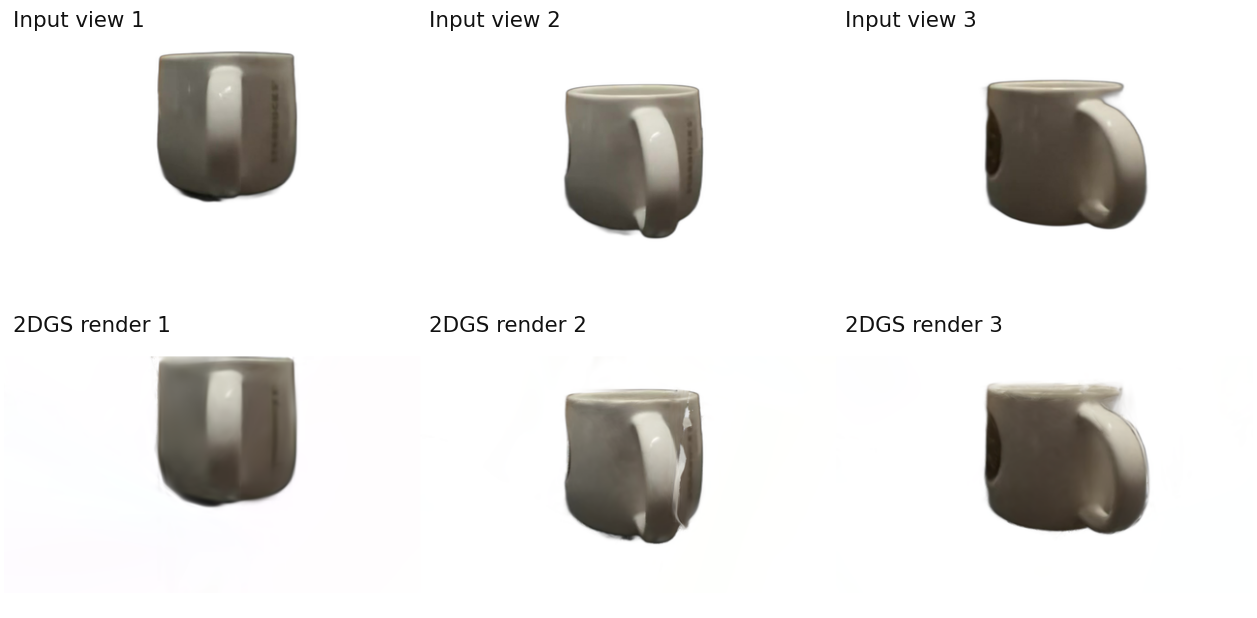
\includegraphics[width=0.98\linewidth]{figures/task1_a_views.png}
\caption{物体 A 的白背景 30k 2DGS 同相机对照。上排是 COLMAP 注册后的真实前景图，下排是对应相机的 2DGS 渲染。}
\label{fig:a_views}
\end{figure*}

\begin{figure}[t]
\centering
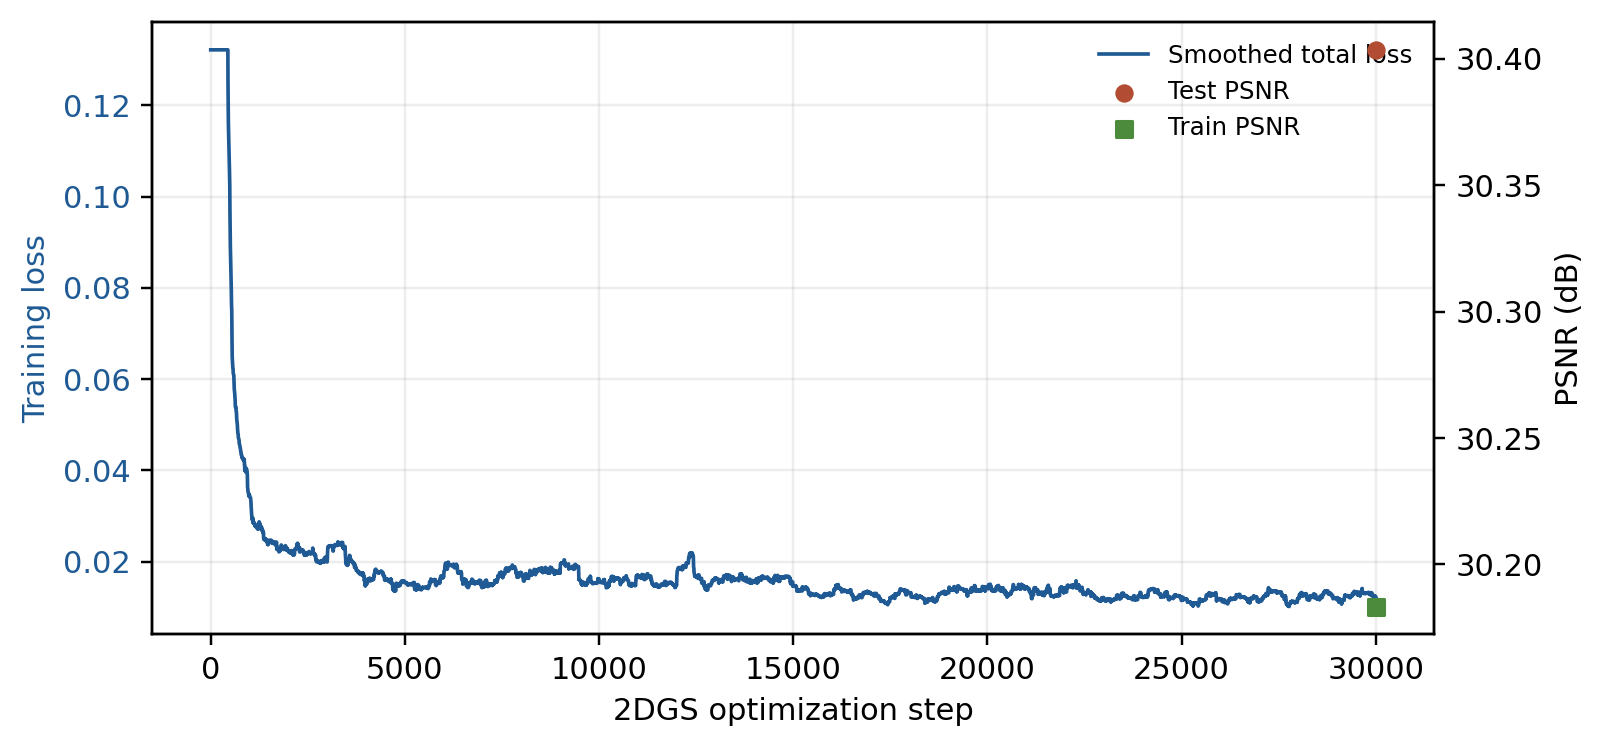
\includegraphics[width=\linewidth]{figures/task1_a_training_curve.png}
\caption{A 的 2DGS 总损失和 30k train/test PSNR。曲线直接读取正式模型 TensorBoard event。}
\label{fig:acurve}
\end{figure}

\subsubsection{失败实验}

部分图片与视频在手部遮挡、焦距、曝光、背景及物体姿态上差异明显，没有稳定注册到同一模型，故只作定性参考。更关键的失败发生在长视频：相邻帧 550--553 的变化确实很小，但局部连续不保证数百次位姿累积后仍能正确闭环。白色釉面缺少稳定 SIFT 特征，镜面高光随视角移动，杯身又近似对称；COLMAP 会优先利用背景或偶然高光，最终把一部分相机放进错误坐标分支。强行使用 762 个注册结果时，2DGS 出现重影、分叉表面和远处浮点。

最终 469 相机的方位覆盖按相机中心绕重建焦点统计约为 281.6°，最大未覆盖区间约 78.4°。因此，输出 360 帧转盘只代表对可靠注册轨迹进行致密插值，不代表获得真实完整 360°。独立渲染主要停留在训练相机流形附近，效果较好；kitchen 漫游相机则会进入覆盖缺口，从侧后方观察只被少数视角约束的杯壁，于是出现孔洞、浮面和高光错误。这解释了“单独看可用、放入场景后变差”的表面矛盾。

融合也经历了三次修正。最初直接旋转原始 2DGS，少量长轴尺度极端的各向异性 surfel 在未见方向下投影为白射线。随后把所有 rotation 重置为单位四元数、尺度改为统一圆盘、opacity 设为 0.24 并清零高阶 SH；射线消失，但杯体表面和陶瓷视角相关外观同时被破坏。该补丁现已废除。正式方案把 66136 个中心投影到 469 个前景 mask；可见次数、至少 5 个前景命中和不低于 0.70 的命中率先给出几何支持，再叠加有限值与 opacity $\geq0.02$ 条件，正式 PLY 实际保留 42800 个中心。随后用固定中心、半径和源坐标基完成相似变换；渲染时再删除归一化长轴超过物体半径 0.12 或各向异性超过 25 的异常 footprint。其余 opacity、两个切向尺度、surfel rotation、DC 与三阶 SH 均保留，SH 系数还随刚体旋转同步换基。该方案去除了渲染过程中产生大量白射线的问题，但不会伪造表面，故最终结果能看到未角度物体资产缺失。

\subsection{物体 B：DreamFusion/SDS 汉堡}

物体B曾尝试选择多种方案。最初的交通锥受薄底板、尖端和低分辨率共同影响，出现破面和轮廓塌缩；随后尝试的蓝色几维鸟能形成单体轮廓，但语义不稳定、细节不足，只作为失败对照保留。正式 B 改为 threestudio ``a delicious hamburger''。配置严格使用 \texttt{stable-diffusion-guidance}、Stable Diffusion 1.5、\texttt{weighting\_strategy=sds}、$\lambda_{\mathrm{SDS}}=1$、guidance scale 100、seed 0；negative prompt 为空，Perp-Neg 关闭，没有使用 SDI、VSD、Zero123 或输入图像。

训练每 200 步保存 RGB、normal 与 opacity 验证图，CSV、TensorBoard 与 W\&B offline run 同步记录 SDS loss 和梯度范数。图~\ref{fig:bcurve} 是训练时真实记录，图~\ref{fig:bprogress} 展示轮廓从粗糙颜色块逐步收敛为上下两层面包、蔬菜和肉饼。最终使用 density isosurface 自动阈值导出 UV、MTL 与 diffuse 纹理 OBJ。SDS 仍存在典型限制：几何表面颗粒较粗，配料边缘会形成毛刺，且 SD1.5 的二维先验不能保证所有背面纹理一致。此外，训练过程中保存的验证视图（图~\ref{fig:bprogress}）与最终导出的 mesh 转盘（图~\ref{fig:independent} 中 B 列）在视觉质量上存在可感知的差异，前者明显优于后者。这一现象并非训练过拟合或渲染参数错误，而是 NeRF 体渲染与 OBJ 漫反射表面之间的表示鸿沟。SDS 在训练期间通过 NeRF 密度场进行体渲染，SD1.5 的评分梯度不仅影响几何，还会引入视角相关的光照效果——高光、色彩饱和度和局部阴影被隐含地编码进密度场和视角相关颜色中，使训练视图呈现出更丰富的视觉层次。当使用 density isosurface 提取等值面并自动展开 UV 后，体渲染的视角相关外观被压平成单一的漫反射纹理（\texttt{texture\_kd.jpg}），视角依赖的光泽和阴影全部丢失。转盘脚本再以简单 diffuse 光照渲染此 OBJ，获得的仅是漫反射 albedo 在均匀环境光下的表现，与 SDS 训练时 SD 先验引导的体积渲染在色彩和立体感上存在天然的不可逆差距。这一差距的根源在于 DreamFusion 的隐式表示不是为 mesh 导出设计的——训练中的视觉质量来自体积散射和视角相关颜色的共同作用，而导出过程只保留了等值面几何和漫反射纹素。

\begin{figure}[t]
\centering
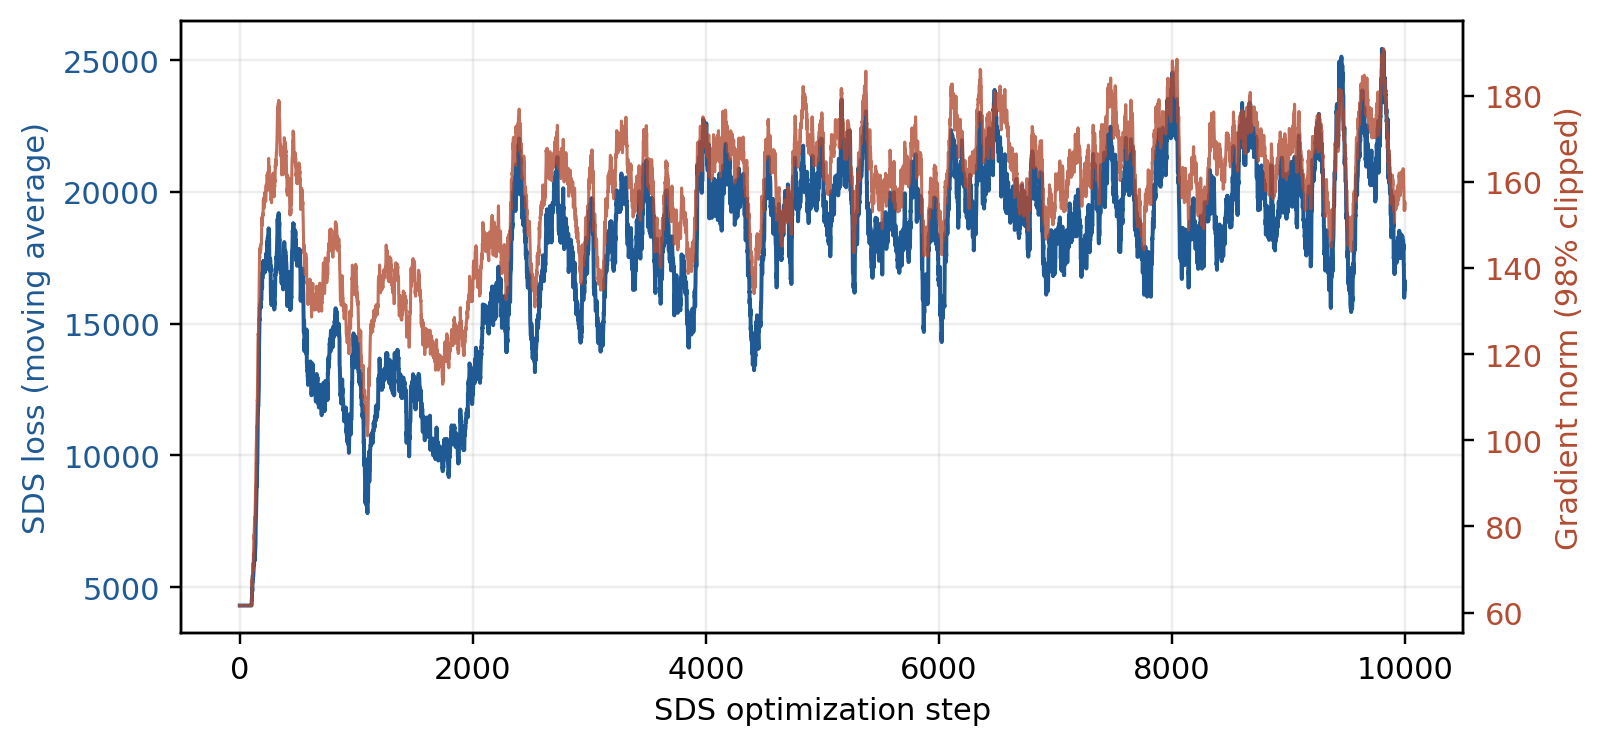
\includegraphics[width=\linewidth]{figures/task1_b_training_curve.png}
\caption{汉堡的 SDS loss 与梯度范数记录}
\label{fig:bcurve}
\end{figure}

\begin{figure*}[t]
\centering
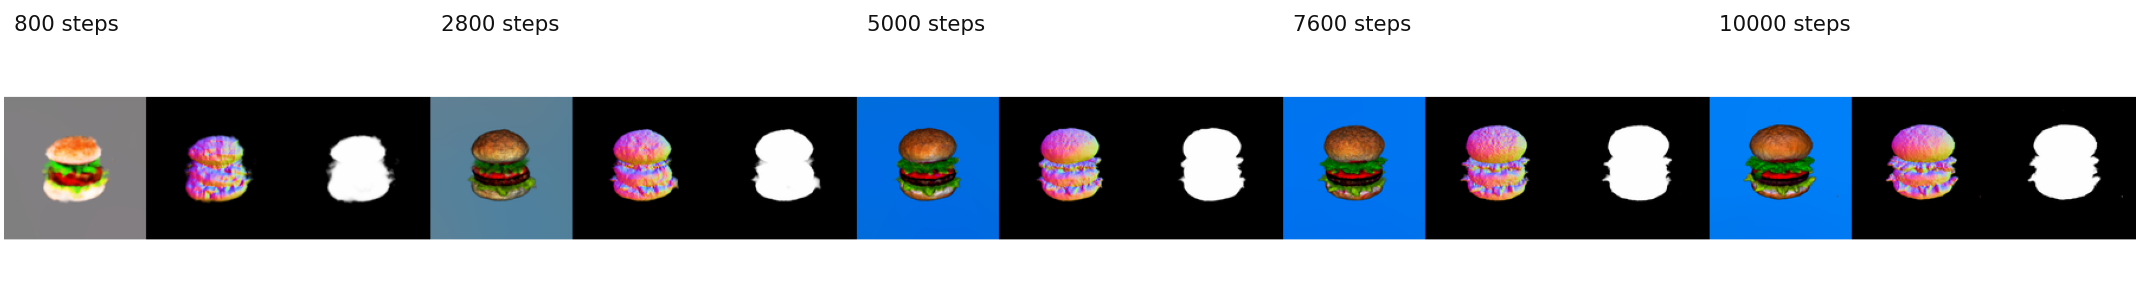
\includegraphics[width=0.98\linewidth]{figures/task1_b_progress.png}
\caption{汉堡在不同优化步数的验证视图。白色图为 opacity，彩色法线用于检查几何连续性}
\label{fig:bprogress}
\end{figure*}

\subsection{物体 C：Magic123 v5 与背面不确定性}

物体 C 以题目给定手柄照片为输入，正式 OBJ 来自 Magic123 的 SD 与 Zero123 双先验优化和 DMTet fine 网格。早期版本出现两个相背正面的 Janus 结构；v5 调整先验权重后形成单一连续手柄，侧面厚度正常，正面轮廓和按键可读。后续 v6 试图进一步强化背面约束，却使 fine 阶段形状和纹理退化，因此正式结果回退到 v5。图~\ref{fig:cversions} 保留了这一选择证据。背面没有真实观测，仍存在生成式纹理和弱几何。

手柄背面出现类正面按钮的纹理伪影，根源在于 SD 1.5 作为二维扩散模型不具备对"白色塑料手柄背面"的精确视觉理解。当 Zero123 从不可见方向采样时，SD 先验倾向于将训练集中最常见的"手柄正面"纹理模式外推到背面，即使 \texttt{dir\_texts\_neg} 提供视角上下文也只能缓解而无法根除。部分渲染中观察到的蓝色失真则来自 SD 的色温偏差：SD 1.5 训练数据中常见的蓝灰色调在被 SDS 梯度反复强化后，在无强观测约束的背面和侧边缘区域形成可见的冷色偏移。这些区域恰好也是几何最薄弱处——DMTet 在有限分辨率（$128^3$）下用四面体网格表达曲面时，网格面在曲率较大的握把过渡处产生可感知的阶梯感；SDS 的随机梯度噪声进一步在表面叠加了高频波动，使最终 mesh 尽管在背面尽量恢复了手柄背面的真实几何凹陷构造，却缺乏真实塑料手柄的光滑连续感，出现部分区域凹陷不齐的情况。

鉴于 v5 训练需消耗大量时间，且逐一尝试 prompt、$\lambda_z$ 和 guidance scale 的排列组合需要在每次完整训练后检验背面，计算成本过高，超出可支配资源，未继续对更高分辨率的 DMTet 或额外视图条件做进一步探索，同理，对物体A、B也如此。

\begin{figure*}[t]
\centering
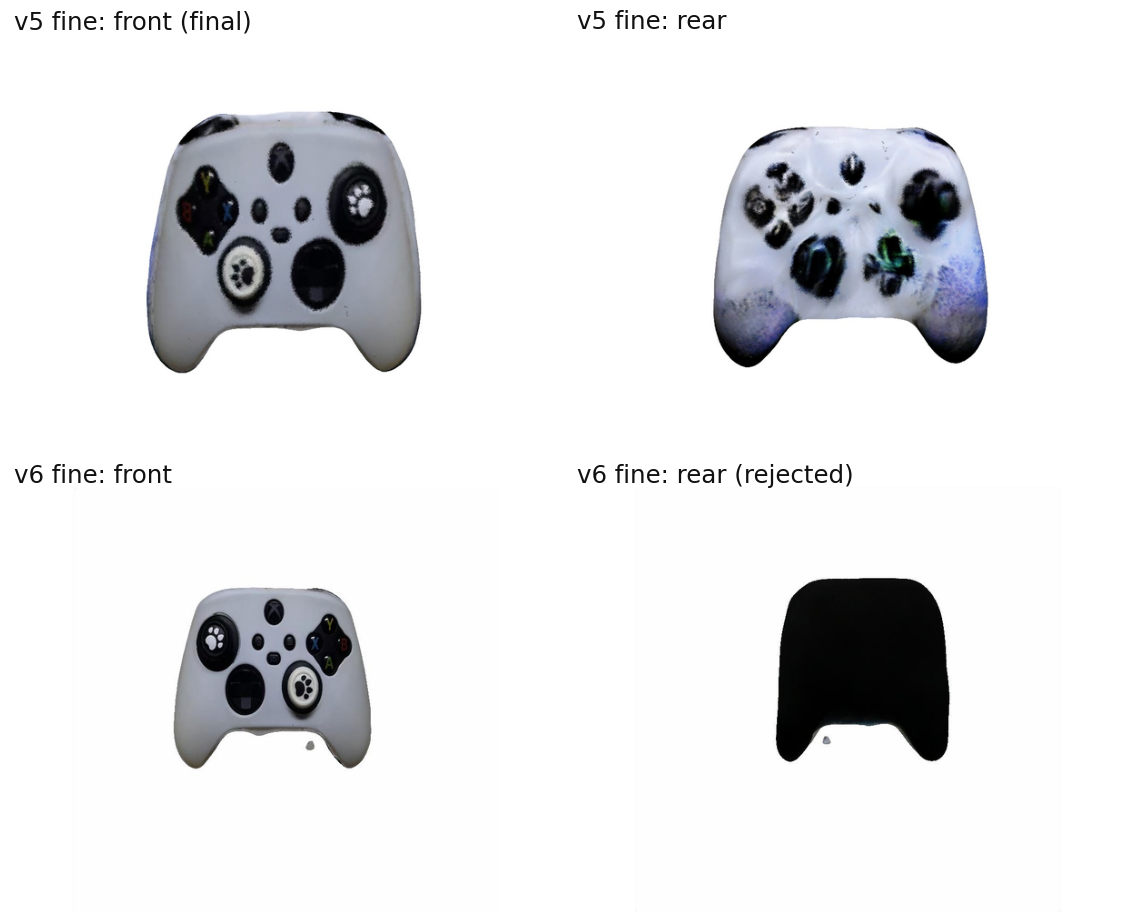
\includegraphics[width=0.96\linewidth]{figures/task1_c_versions.png}
\caption{C 的 v5/v6 正面与背面对照。v5 fine 为正式资产；v6 在不可见背面出现更严重的黑化与细节退化，因此被拒绝。}
\label{fig:cversions}
\end{figure*}

\begin{figure}[t]
\centering
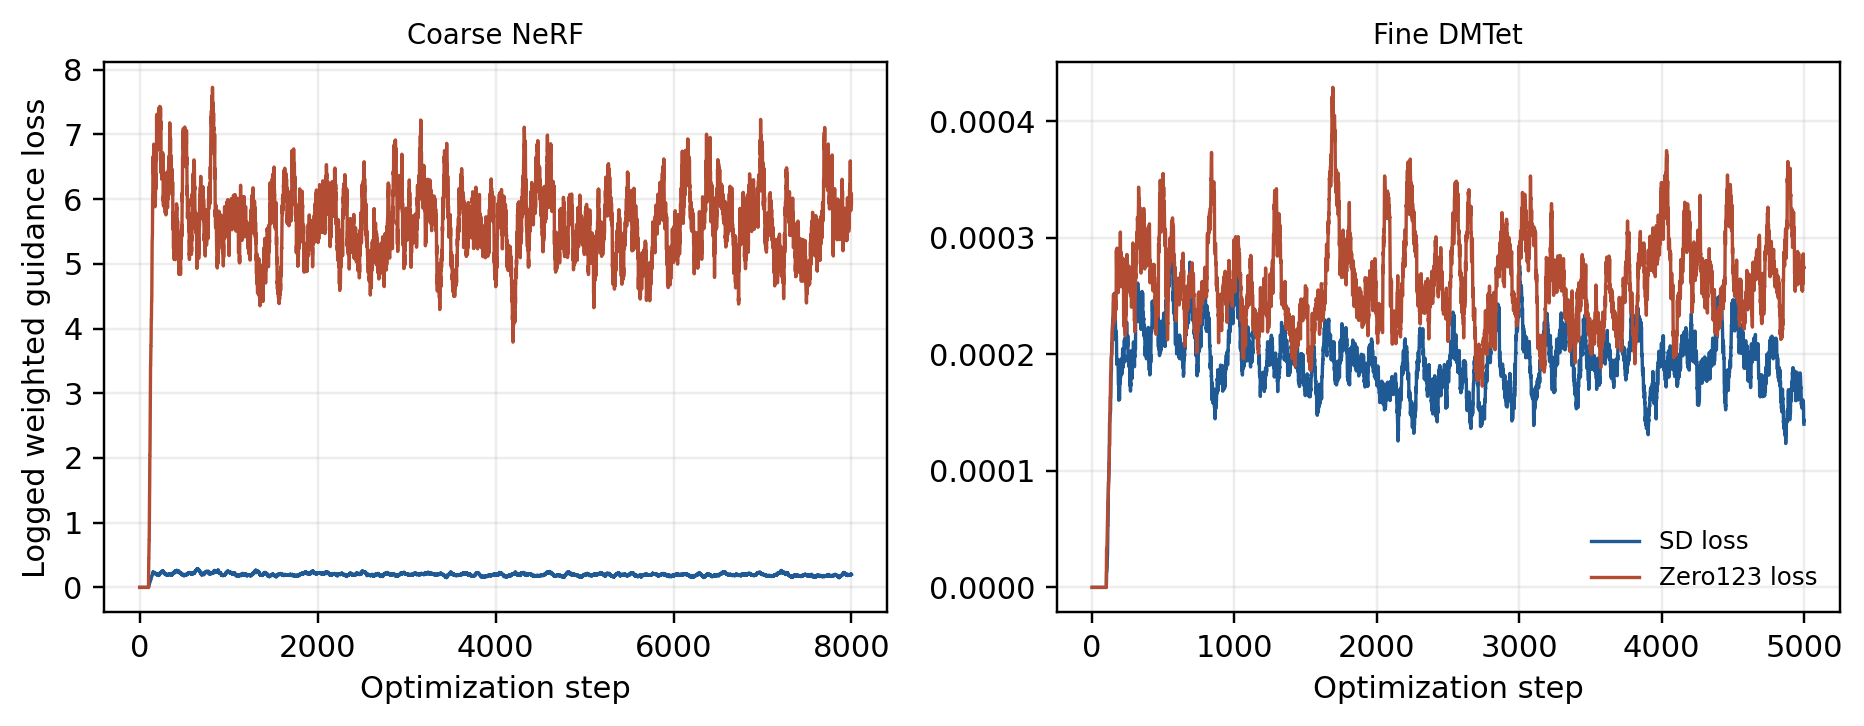
\includegraphics[width=\linewidth]{figures/task1_c_training_curve.png}
\caption{Magic123 v5 coarse/fine 阶段记录的 SD 与 Zero123 加权 guidance loss。}
\label{fig:ccurve}
\end{figure}

\begin{figure*}[t]
\centering
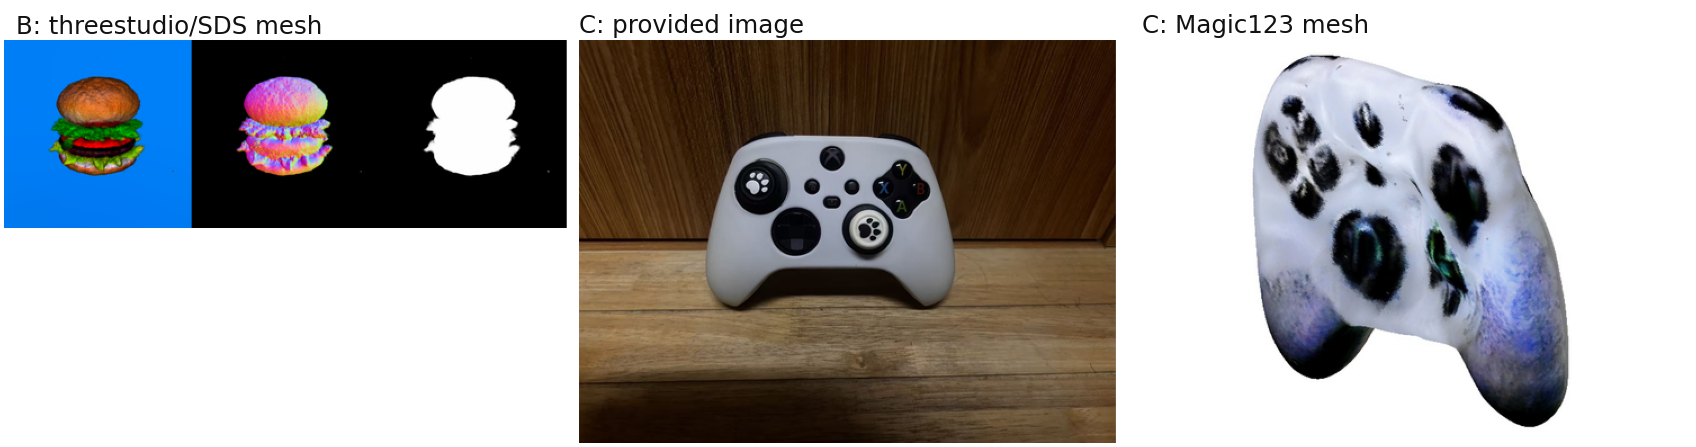
\includegraphics[width=0.98\linewidth]{figures/task1_generated_assets.png}
\caption{题目指定生成路线的实际产物。左：10000 步纯 SDS 汉堡；中：C 的输入图；右：Magic123 v5 fine 网格。}
\label{fig:generated}
\end{figure*}

\subsection{统一表达与合并渲染}

背景使用 Mip-NeRF 360 kitchen，2DGS 模型训练 7000 次迭代，加载 279 个相机，Gaussian PLY 约 180.7 MB。2DGS 以有方向的平面 Gaussian 建模表面，并通过 ray--splat intersection 获得视角一致的深度和法线~\cite{huang20242dgs}。SuGaR 进一步表明，将 Gaussian 约束到表面可以支持可编辑 mesh 与 Gaussian 渲染的结合~\cite{guedon2024sugar}。受此思路启发，本项目实现确定性的 mesh-to-2D-Gaussian 转换，但没有使用 SuGaR 的训练或联合优化。

对 B/C，设三角形 $f$ 的面积为 $A_f$，总采样数为 $N$。先按 $A_f/\sum_j A_j$ 分配样本，再用重心坐标在三角形内部均匀采样。每个样本的局部法向为该三角形单位面法线 $\mathbf n_f$，通过将 Gaussian 局部 $+Z$ 轴旋转至 $\mathbf n_f$ 得到四元数。切向标准差按
\[
s_f=\alpha\sqrt{\frac{\sum_j A_j}{\pi N}}
\]
设置，其中 $\alpha=1.45$，从而得到贴附 mesh 表面的 2D 椭圆盘。B 使用导出的 UV、MTL 与 \texttt{texture\_kd.jpg}；C 只读取 OBJ 的 UV 和 \texttt{albedo.png}，不再把正面输入图投影到侧面或背面。

A 经过前景支持和异常 footprint 过滤后，与 B/C 的采样 Gaussian 一起转换为与背景完全相同的参数：中心、SH/DC 颜色、opacity、两个切向尺度和四元数旋转。A 的变换是固定的刚体相似变换，不进行联合优化；尺度只在两个切向 log-scale 上增加同一个全局缩放量，旋转以矩阵左乘更新，三阶 SH 通过 128 个球面采样方向求基变换。随后直接拼接到背景 \texttt{GaussianModel} 的 tensor，每帧只调用一次官方 2DGS rasterizer，因此 A/B/C 与背景共享相机矩阵、透视投影、alpha compositing 和深度排序。

材质统一存在清晰边界。OBJ 的 UV/albedo 能转成视角无关的 diffuse/radiance 颜色，但粗糙度、金属度、镜面 BRDF、透明和折射参数没有被当前 2DGS shader 表达。陶瓷杯的高光保留在 A 已学习的 SH 中；B/C 则主要保留 albedo 外观。这是一种统一的可见表面表示，不是完整 PBR 材质迁移。

布局严格沿用已验收参数：公共 scene scale 为 0.072，forward/up 偏移为 $0/-0.12$；A/B/C 半径均为 0.34，角度为 $-0.8/0.8/1.8$ rad，高度为 $0.20/0.25/0.25$，缩放为 $0.95/1.45/1.30$，yaw 为 $-1.20/0.25/-0.30$。A 额外使用 $\pi/2$ pitch 修正源相机基与桌面基的轴向差；位置参数不变。相机沿 kitchen 原路径旋转，最终输出 360 帧 H.264/yuv420p MP4。图~\ref{fig:fusionevolution} 对比旧插入、12 帧表面对齐预览和正式结果。

\begin{figure*}[t]
\centering
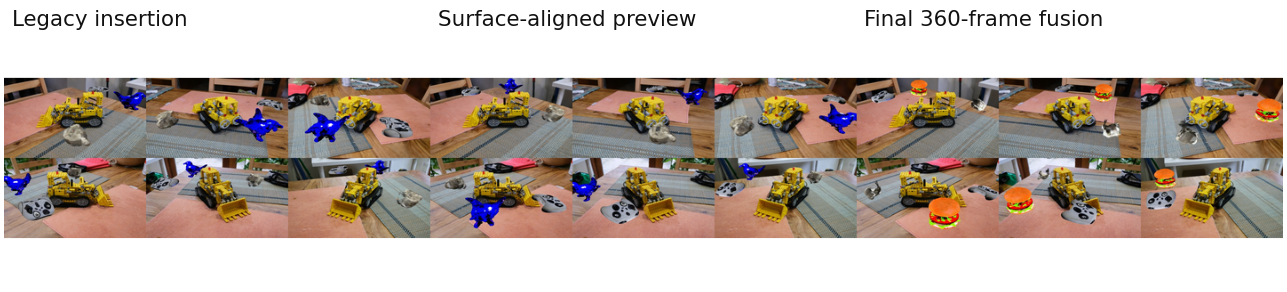
\includegraphics[width=0.98\linewidth]{figures/task1_fusion_evolution.png}
\caption{融合方式演变。旧方案存在二维代理、错误纹理投影或方向问题；表面对齐预览验证统一 Gaussian 路线；正式结果替换为汉堡并保持固定布局。}
\label{fig:fusionevolution}
\end{figure*}

\begin{figure*}[t]
\centering
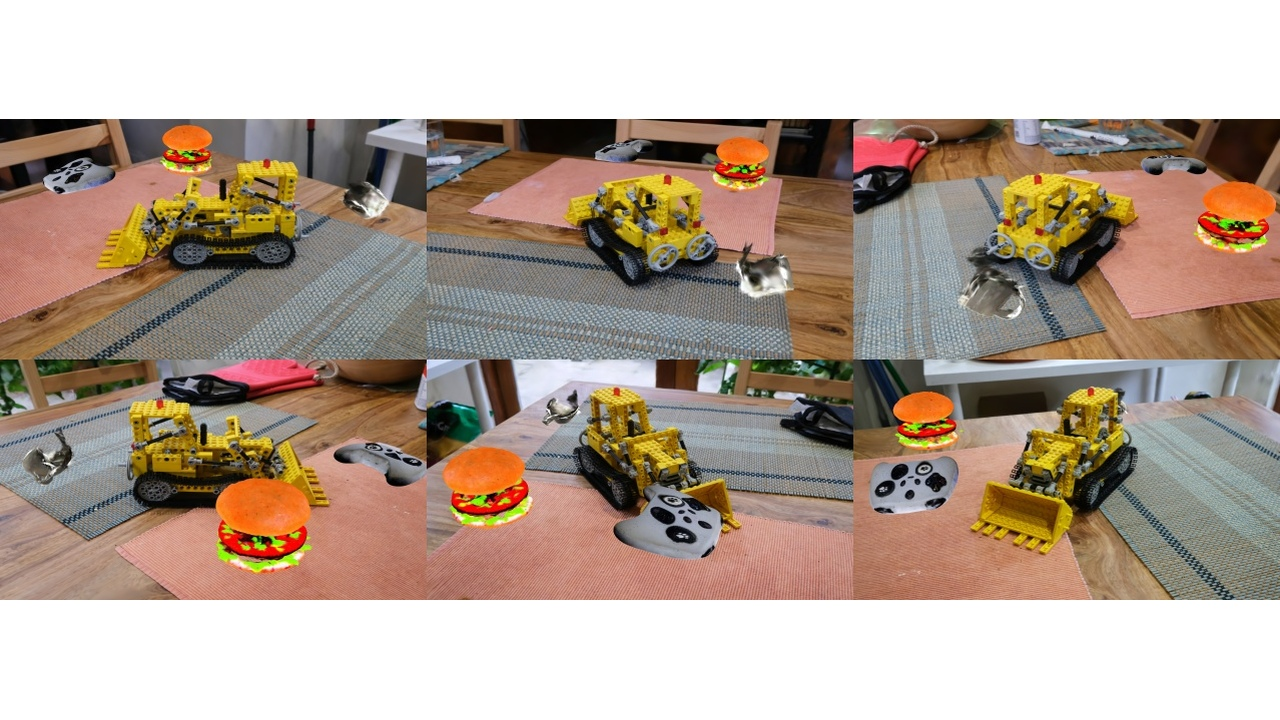
\includegraphics[width=0.98\linewidth]{figures/task1_scene_contact.jpg}
\caption{最终 360 帧融合视频的六帧抽样。背景与 A/B/C 均由同一 2DGS rasterizer 完成深度排序和 alpha 合成。}
\label{fig:scene}
\end{figure*}

\begin{figure*}[t]
\centering
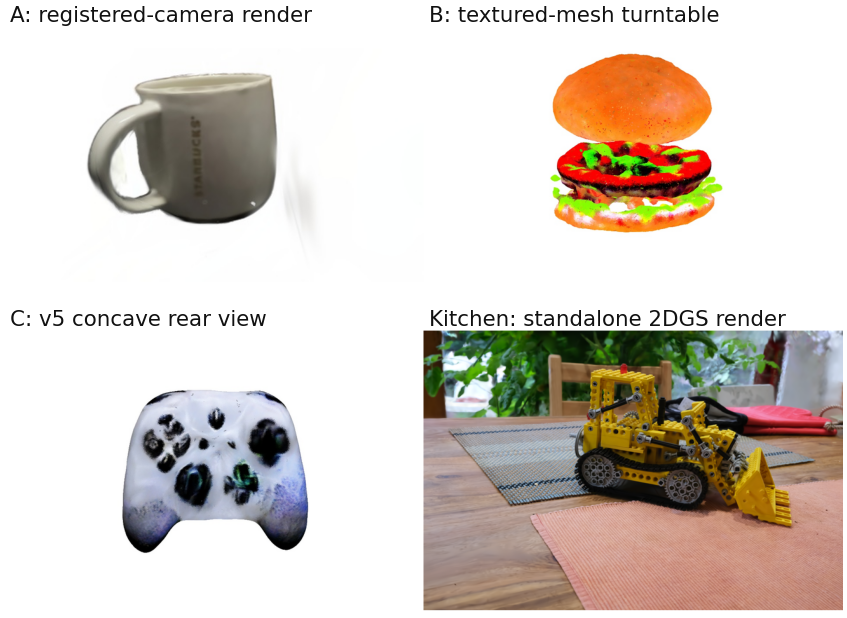
\includegraphics[width=0.98\linewidth]{figures/task1_independent_quality.png}
\caption{融合前的独立质量检查：A 的注册轨迹渲染、B 的 mesh 转盘、C 的 v5 凹陷背面视角和 kitchen 的独立 2DGS 相机渲染。该图用于区分资产生成误差与融合视角外推误差。}
\label{fig:independent}
\end{figure*}

\subsection{三种生成路线的质量比较}

\begin{table*}[t]
\centering
\caption{三种题目指定路线的质量与代价比较。定量指标只在有真实测试视图的 A 上报告；B/C 的不可见面没有 ground truth，采用多视图一致性和人工可读性分析。}
\label{tab:t1compare}
\small
\begin{tabular}{p{1.6cm}p{2.7cm}p{2.8cm}p{2.7cm}p{2cm}p{2.4cm}}
\toprule
路线 & 几何准确度 & 纹理细节 & 不可见面 & 计算耗时 & 主要误差 \\
\midrule
多视角 A & 观测区最强；test PSNR 30.40 dB & 杯沿和高光可见，但视角依赖强 & 78.4° 可靠方位缺口 & 训练 8m55s；COLMAP 未计时 & 低纹理、反光、漂移分支、未见方位 \\
文本 B & 汉堡整体层次清楚，但边缘粗糙 & 配料颜色鲜明，局部颗粒化 & 完全由 SD1.5 先验生成 & 训练 38m48s & SDS 毛刺、层间空隙、背面语义一致性 \\
单图 C & 正面和厚度可用 & 正面按钮最佳，背面较弱 & 由 Zero123/SD 推断 & 训练 44m47s；含导出约 51m20s & Janus 风险、背面幻觉 \\
\bottomrule
\end{tabular}
\end{table*}

\textbf{监督信号和可辨识性。}
三条路线最根本的差别在于证据先验。 A 的颜色与几何由 469 个已标定真实视图共同约束，只要某个表面被多个相机看到，其错误会同时破坏多张图像的一致性，因此观测区具有三者中最高的可验证性。B 没有任何特定实例的观测，SDS 只要求随机视角渲染落在文本条件扩散模型的高概率图像区域；“看起来像汉堡”可以由许多互不相同的三维结构实现，所以语义正确不等于几何正确。C 有一张实例图作为强前视约束，同时依赖 Zero123/SD 生成未见视图；它比 B 更能保持目标身份，却仍无法从单张投影唯一确定厚度、背面拓扑和背面纹理。因此三者的信息约束强度是“多视角实例证据 $>$ 单视角实例证据+生成先验 $>$ 纯语义先验”，但这一排序只对真实实例保真成立，不代表最终图像一定更漂亮。

\textbf{真实性、完整性与可感知质量。}
A 在已观测区域的实例真实性最高，却因方位缺口而完整性最低；B 不追求对应现实实例，生成先验可以给出视觉上连续的 360° 表面，因此完整性和类别可读性较强，但真实性没有可比较对象；C 位于两者之间，正面身份真实性较高，背面完整性主要由先验换取。若只看最终转盘，“每个角度都有颜色”的 B/C 容易被误判为优于 A；若评价目标改成“是否忠实复制指定杯子”，则只有 A 的已观测区域有多视图证据。本文因此不把三条路线压缩成单一总分，而分别报告实例保真、视角完整、表面连续和融合后材质保留。这个拆分也解释了为何 A 的数值指标最好而最终场景仍可能最显破损：指标覆盖的是有证据区域，视频会主动穿过最弱的未见区域。

\textbf{纹理细节和几何细节。}
A 的陶瓷高光存储在视角相关 SH 中，训练视角附近可以呈现较自然的光泽，但高光会随错误相机位姿一起被烘入辐射场；当视角越过观测边界时，错误不仅表现为颜色模糊，还会通过过大的 surfel footprint 放大成射线或浮面。B 的鲜艳配料主要来自 SD1.5 的图像先验，颜色可读性高于局部网格质量，属于“纹理语义强、表面度量弱”。C 的输入正面通过已知视图 RGB/mask loss 得到最强保持，侧后面则主要受生成先验控制，呈现“正面细节强、背面可信度低”的不对称。由此不能简单用清晰度判断几何：一个锐利的生成纹理可能贴在错误表面上，而 A 的低纹理白杯即使几何较合理，视觉上也可能不如汉堡醒目。

\textbf{统一表示会以不同方式放大源资产缺陷。}
A 原本就是有方向、带 opacity 和高阶 SH 的 2D Gaussian，刚体相似变换理论上可以保留其已学习外观；实际风险来自训练相机流形之外的 footprint 投影和 SH 外推。因此正式方案保留全部可学习属性，只过滤有明确证据的背景中心与极端 footprint。B/C 从 mesh 转为 2D Gaussian 时，三角形面积和法线能保留表面位置、朝向与漫反射 albedo，却不包含粗糙度、镜面、透明或折射参数；采样密度过低会漏面，footprint 过大则会跨越薄结构并模糊轮廓。换言之，A 的主要融合误差是“视角外推”，B/C 的主要融合误差是“mesh 到 surfel 的离散化和材质降阶”。同一 rasterizer 解决了深度排序和 alpha 合成的一致性，但不会自动消除这些源域误差。

\textbf{误差的传播方式。}
A 的误差链为“低纹理/反光视频 $\rightarrow$ COLMAP 位姿与覆盖缺口 $\rightarrow$ 2DGS 在错误或缺失射线上拟合 $\rightarrow$ 新视角下 footprint 与 SH 外推”；其中相机覆盖是上游瓶颈，事后改 opacity 或重置 rotation 只能掩盖症状并损伤已观测区域。B 的误差链为“文本歧义与 SD1.5 类别先验 $\rightarrow$ SDS 对单视图高概率而非三维一致性优化 $\rightarrow$ density/mesh 毛刺 $\rightarrow$ 面积采样把毛刺忠实转换为 surfel”；提高最终视频分辨率不会修复上游几何。C 的误差链为“单图投影歧义 $\rightarrow$ Zero123/SD 对不可见面猜测 $\rightarrow$ DMTet 固化猜测拓扑 $\rightarrow$ albedo-only Gaussian 化丢失材质响应”。因此三条路线的有效改进位置也不同：A 应优先改善采集和相机注册，B 应改善三维一致性先验或 SDS 优化，C 应增加真实侧后视图或多图条件；单独调融合尺度只适合解决采样孔洞和 footprint 过大，不能补救源资产的语义或拓扑错误。

\textbf{计算耗时。}
日志中 A 的 30000 步 2DGS 训练为 8m55s，但这一数字不含视频拍摄、去背景、COLMAP 匹配、错误分支诊断和人工筛帧；把它与端到端生成时间直接比较会明显低估 A 的数据准备成本。B 的 10000 步训练为 38m48s，无需实例采集，但需要多视角 SDS 反向传播。C 的 coarse/fine 训练分别为 29.28/15.49 分钟，UV 展开和最终 mesh 写出使从首次训练开始到最终导出的日志跨度为 51m20s。C 花费更久仍不能恢复真实背面，A 训练更快却需要昂贵的数据和位姿准备，说明瓶颈由监督信息和优化目标共同决定，而不是 GPU 时间越长质量越高。

\textbf{失败模式与适用场景。}
若目标是复刻一个指定真实物体，且能保证纹理、光照和视角覆盖，多视角 A 最可靠；本实验的杯子恰好违反了“丰富纹理、近 Lambertian、完整环绕”三个条件，因此位姿质量成为上限。若目标是快速获得语义明确、无需对应现实实例的装饰资产，B 的文本 SDS 成本最低，但需要接受局部几何和背面一致性不可验证。若必须保持输入对象身份、又只能采集一张图，C 是折中方案；报告中的 v5/v6 对照表明，增加生成约束并不保证单调改善，不可见面仍应以不确定区域而非重建真值对待。最终场景中三个对象的质量排序也随观察角度改变：A 在注册轨迹附近最好，C 在正面最好，B 的语义在较大角度范围内最稳定，但三者都没有达到完整 PBR 资产的材质一致性。

\section{任务二：CALVIN 上的 ACT}

\subsection{数据子集与模型}

数据来自 Hugging Face 的 \texttt{huiwon/calvin\_task\_ABC\_D}，整理后的复现副本发布于首页所列 Hugging Face 地址。Hub 页面记录的远端压缩文件总量约为 7.81 GB；最初完整下载的 \texttt{data/calvin\_hf} 在本机实测约 13 GB，差异来自 Hub 统计口径、本地缓存、元数据和文件系统开销。原始 LeRobot v3 shard 以 AV1 视频保存两路 $256\times256$ 相机，以 Parquet 保存状态、动作、任务和索引。训练随机访问帧时，AV1 解码成为数据加载瓶颈，因此按完整 episode 解码为 LeRobot \texttt{image} 特征。

子集构建以 23300200022 为主种子，A/B/C/D shard 分别使用 23300200022--23300200025；按各环境原帧数比例随机打乱 episode，只保留完整轨迹，不截断也不生成新样本。最终得到 39.958 GB、369952 帧。体积增长来自把高压缩率 AV1 改成逐帧图像，以磁盘换取稳定读取吞吐。完整选择列表和每个 episode 可在 \texttt{subset\_manifest.json} 中追溯。A+B+C 用于联合训练，D 未参与梯度更新，只用于 zero-shot 评价。

策略采用 LeRobot ACT。输入包括 15 维机器人状态、$256\times256$ 的静态相机图像和腕部相机图像；输出为 7 维动作 $(\Delta x,\Delta y,\Delta z,\Delta r,\Delta p,\Delta y,g)$。视觉主干为 ImageNet 预训练 ResNet-18，Transformer 隐藏维度 512、8 个注意力头、4 层编码器、1 层解码器，VAE latent dimension 为 32，KL 权重为 10。Action chunk size 与 \texttt{n\_action\_steps} 均为 10，即一次视觉观测生成并排队执行 10 个动作。当前配置的 \texttt{temporal\_ensemble\_coeff} 为空，没有利用相邻时刻重叠预测进行 temporal ensembling；因此本文分析的是固定 10 步开环 action chunk，而不是每一步重新查询并融合多个 chunk 。

\begin{table*}[t]
\centering
\caption{Task2 的受控 ACT 训练设置。}
\label{tab:t2settings}
\scriptsize
\resizebox{\textwidth}{!}{%
\begin{tabular}{lrrrrlllll}
\toprule
模型 & Batch & Step & Seed & Chunk & Optimizer & LR / backbone LR & Schedule & Loss \\
\midrule
B-only & 256 & 10000 & 1000 & 10 & AdamW, wd $10^{-4}$ & $10^{-4}/10^{-5}$ & 500 warmup + cosine & Action L1 + $10\cdot$KLD \\
A+B+C & 256 & 10000 & 1000 & 10 & AdamW, wd $10^{-4}$ & $10^{-4}/10^{-5}$ & 500 warmup + cosine & Action L1 + $10\cdot$KLD \\
\bottomrule
\end{tabular}
}
\end{table*}

为隔离训练数据范围，两组以同一随机种子独立初始化策略层，并加载同一 ImageNet ResNet-18 预训练主干，随后训练 10000 step；每步 256 个样本，共处理 256 万个训练样本。两组均使用 500-step linear warmup，再从 $10^{-4}$ cosine decay 到 $10^{-5}$；AdamW、梯度裁剪、图像预处理和 checkpoint 频率完全相同。warmup 抑制训练初期 VAE 与视觉主干联合优化的梯度冲击，后期衰减则在不增加 step 的情况下提高收敛质量。B-only 数据含 92581 帧，相当于约 27.65 次数据遍历；A+B+C 含 277678 帧，相当于约 9.22 次联合数据遍历。

图~\ref{fig:training} 直接解析两次正式训练的 stdout，每 20 step 记录一次训练 loss，并采用 15 点移动平均。原始记录同时导出为 W\&B offline runs，完整 D 指标则单独标注为 post-training evaluation，避免把教师强制评价伪称为训练期在线验证。

\begin{figure}[t]
\centering
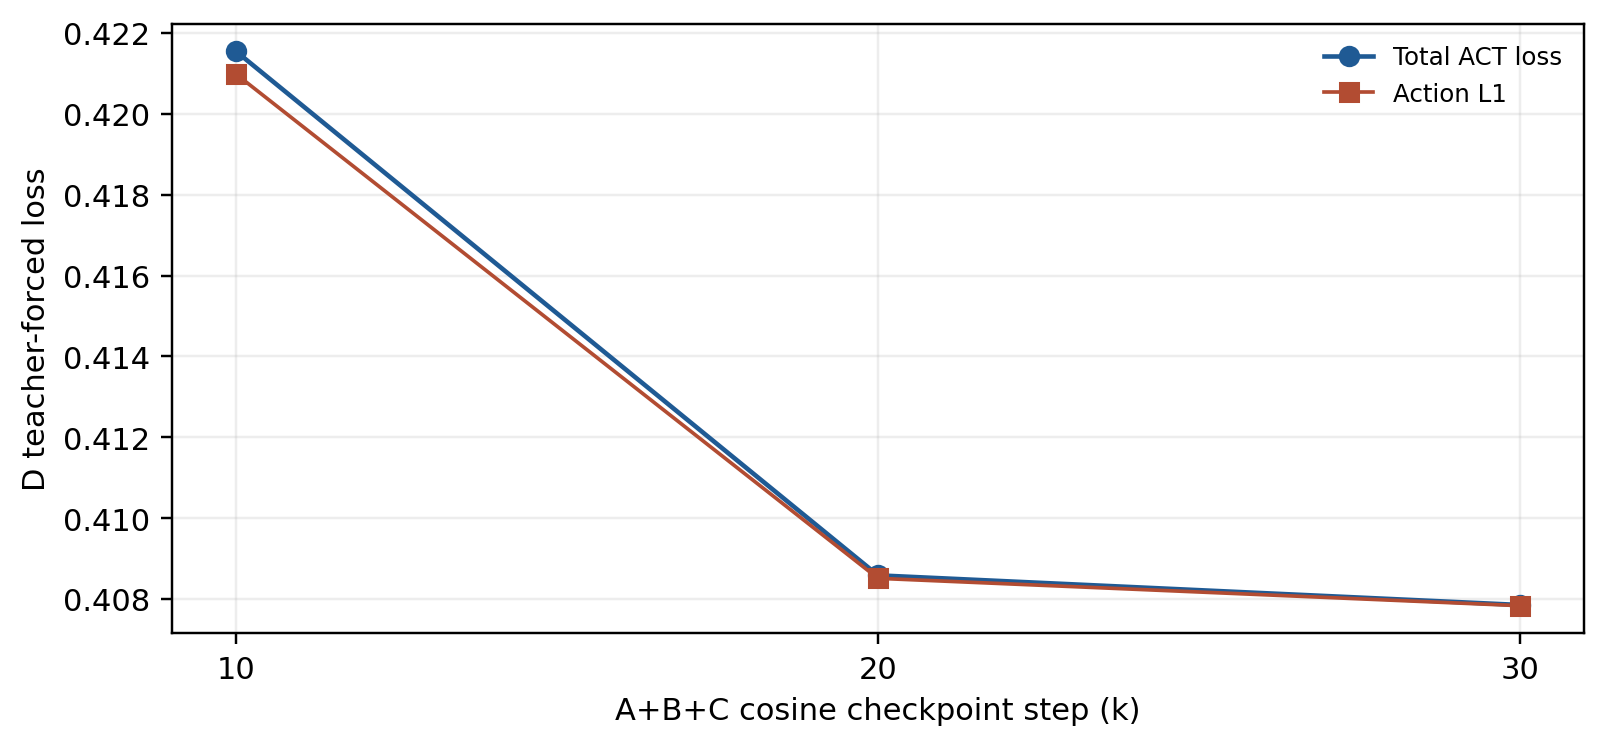
\includegraphics[width=\linewidth]{figures/task2_training_curve.png}
\caption{公平 10k 协议下 B-only 与 A+B+C 的训练 loss。两条曲线来自相同日志频率和相同优化设置。}
\label{fig:training}
\end{figure}

\subsection{评价协议与补充指标}

主结果使用同一脚本、同一 D 根目录和 batch size 256，对完整 D shard 的 92274 个样本计算教师强制 ACT loss。为了直接研究 Action Chunking，另取 B 和 D 各自按数据顺序排列的前 64 个 batch，每个 batch 128 个样本，即每个环境 8192 个样本；两个模型使用完全相同的样本顺序。受控实验调用 \texttt{predict\_action\_chunk} 得到 $\hat{\mathbf a}_{i,1:10}$，并定义分块位置误差
\[
E_k=\frac{1}{7N}\sum_{i=1}^{N}\left\lVert
\hat{\mathbf a}_{i,k}-\mathbf a_{i,k}\right\rVert_1 .
\]
尾部放大率定义为
\[
R_{\mathrm{tail}}=\frac{(E_8+E_9+E_{10})/3}{(E_1+E_2+E_3)/3}.
\]
$R_{\mathrm{tail}}>1$ 表示同一视觉条件下越远期动作越不可靠。除 L1 外，还计算机械臂前六维动作的余弦相似度、夹爪符号准确率、相邻动作差分 L1，以及预测/真实时序变化比
\[
R_{\mathrm{var}}=
\frac{\mathbb{E}\lVert\hat{\mathbf a}_{k+1}-\hat{\mathbf a}_{k}\rVert_1}
{\mathbb{E}\lVert\mathbf a_{k+1}-\mathbf a_{k}\rVert_1}.
\]
$R_{\mathrm{var}}\ll1$ 表示输出虽然平滑，但可能把真实动作变化过度抹平。两个模型在 clean D 上的差值按 batch 配对，并以固定随机种子进行 5000 次 bootstrap，报告 95\% 置信区间和配对效应量 $d_z$。

视觉偏移实验保持机器人状态和动作标签不变，只修改同一帧的两路图像。外观变化包括 0.55 倍亮度、1.35 倍亮度、低对比度和暖色偏移；图像损坏包括 $9\times9$ 均值模糊和标准差 0.08 的高斯噪声；空间变化包括水平 16 像素、垂直 $-8$ 像素的相机平移和中央 32\% 区域遮挡；相机消融则分别把静态或腕部相机替换为常量灰图。该分解与 Xie 等人将光照、相机位置等因素分别测量的视觉模仿泛化方法一致~\cite{xie2023generalization}。预测漂移定义为扰动图像与 clean 图像在同一状态上输出 chunk 的平均 L1，可分离“模型对图像变化的敏感性”和“动作标签本身的难度”。

\subsection{完整 D 的 zero-shot 动作误差}

\begin{table*}[t]
\centering
\caption{保留 D 环境上的统一教师强制评价。所有值越低越好。}
\label{tab:offline}
\small
\begin{tabular}{lrrrrr}
\toprule
训练设置 & Step & Schedule & Total loss & Action L1 & KLD \\
\midrule
B only & 10k & cosine & 0.509554 & 0.509418 & 0.00001358 \\
\rowcolor{bestrow}
A+B+C & 10k & cosine & \textbf{0.432869} & \textbf{0.432757} & \textbf{0.00001120} \\
\bottomrule
\end{tabular}
\end{table*}

\begin{figure}[t]
\centering
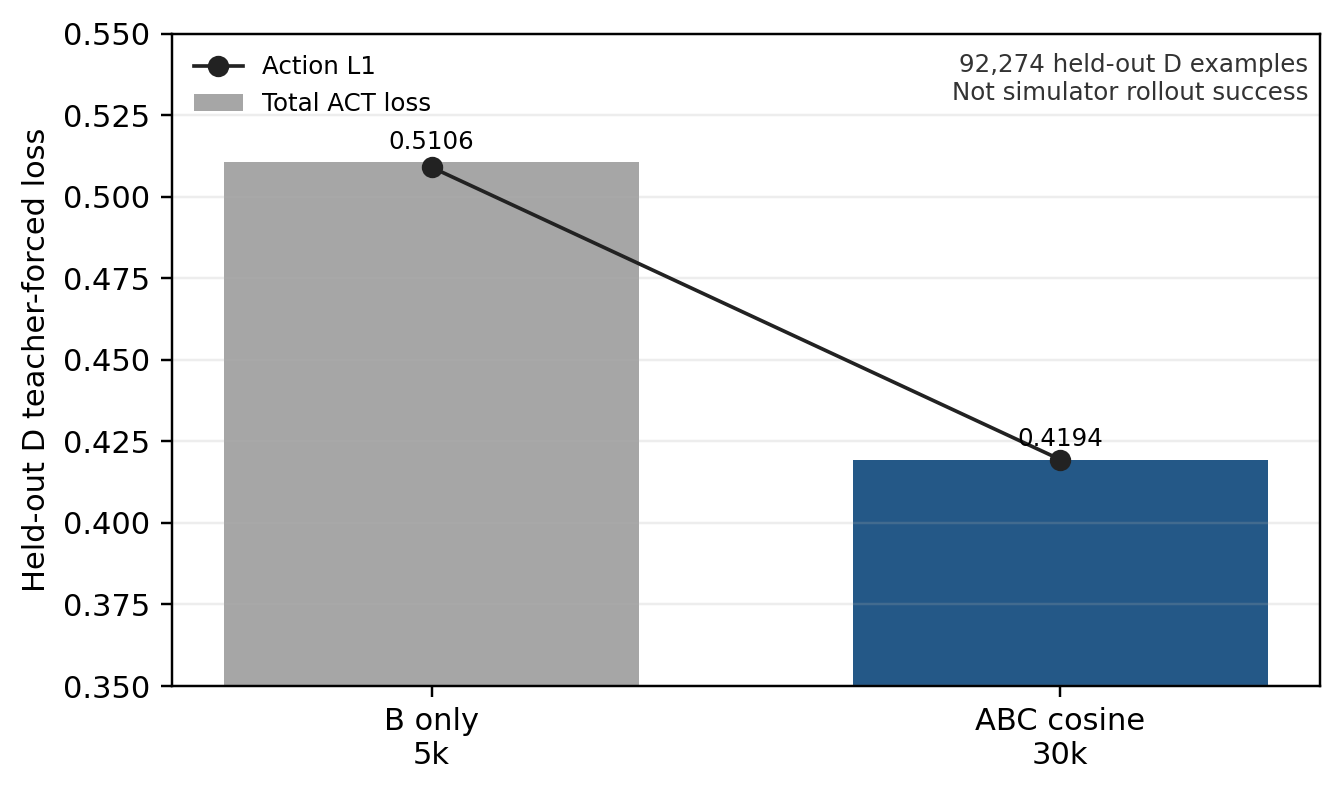
\includegraphics[width=\linewidth]{figures/task2_offline_eval.png}
\caption{完整 D shard 的 zero-shot 动作误差评价。柱为总 ACT loss，折线为 Action L1。图中明确标注该结果不是 simulator rollout success。}
\label{fig:offline}
\end{figure}

表~\ref{tab:offline} 和图~\ref{fig:offline} 来看，在网络、优化器、batch、训练步数、调度器和随机种子全部对齐后，A+B+C 相对 B-only 将 Action L1 降低
\[
\frac{0.509418-0.432757}{0.509418}\times100\%=15.05\%,
\]
总损失同样降低 15.05\%。配置审计逐项比较两个 \texttt{train\_config.json}，确认唯一允许的差异是训练数据从 B 扩展为 A+B+C，因此该结果可以解释为固定训练成本下多环境数据带来的跨环境收益。受控 8192 样本子集上，B-only 与 A+B+C 的 clean D L1 分别为 0.5374 和 0.4627，下降 13.90\%，方向与完整 D 一致；幅度差异来自有序子集与完整分布的组成不同。

\subsection{跨环境差距与统计显著性}

\begin{table}[t]
\centering
\caption{同一 8192 样本协议下的 B$\rightarrow$D 泛化差距。}
\label{tab:crossenv}
\small
\begin{tabular}{lrrrr}
\toprule
模型 & B L1 & D L1 & 绝对差 & 相对差 \\
\midrule
B-only & 0.1480 & 0.5374 & 0.3894 & 263.07\% \\
A+B+C & 0.2039 & 0.4627 & \textbf{0.2588} & 126.95\% \\
\bottomrule
\end{tabular}
\end{table}

表~\ref{tab:crossenv} 显示，B-only 在训练域 B 上更低，这是其反复暴露于单一环境的预期结果；A+B+C 牺牲部分 B 域拟合，换取更好的未见 D 表现。其绝对 B$\rightarrow$D 差距由 0.3894 降为 0.2588，缩小 33.5\%。对 64 个 clean-D batch 做配对统计，B-only 减 A+B+C 的平均 L1 差为 0.07493，95\% bootstrap CI 为 $[0.05211,0.09941]$，不跨 0，配对效应量 $d_z=0.78$。因此多环境训练的收益不是由少数 batch 拉动，而是稳定的中等偏大效应。

\subsection{Action Chunking 的分块位置鲁棒性}

ACT 的原始动机是一次建模动作序列，以减少逐步行为克隆中的误差累积并保持动作一致性~\cite{zhao2023act}。图~\ref{fig:chunk} 左侧显示，A+B+C 在全部 10 个位置均低于 B-only。B-only 的 $E_1/E_{10}$ 为 0.5402/0.5574，A+B+C 为 0.4685/0.4824；对应 $R_{\mathrm{tail}}$ 分别为 1.020 和 1.018。即使在未见 D 中，10 步 chunk 的尾部误差也只比头部高约 2\%，没有出现随 $k$ 单调爆炸。

\begin{figure*}[t]
\centering
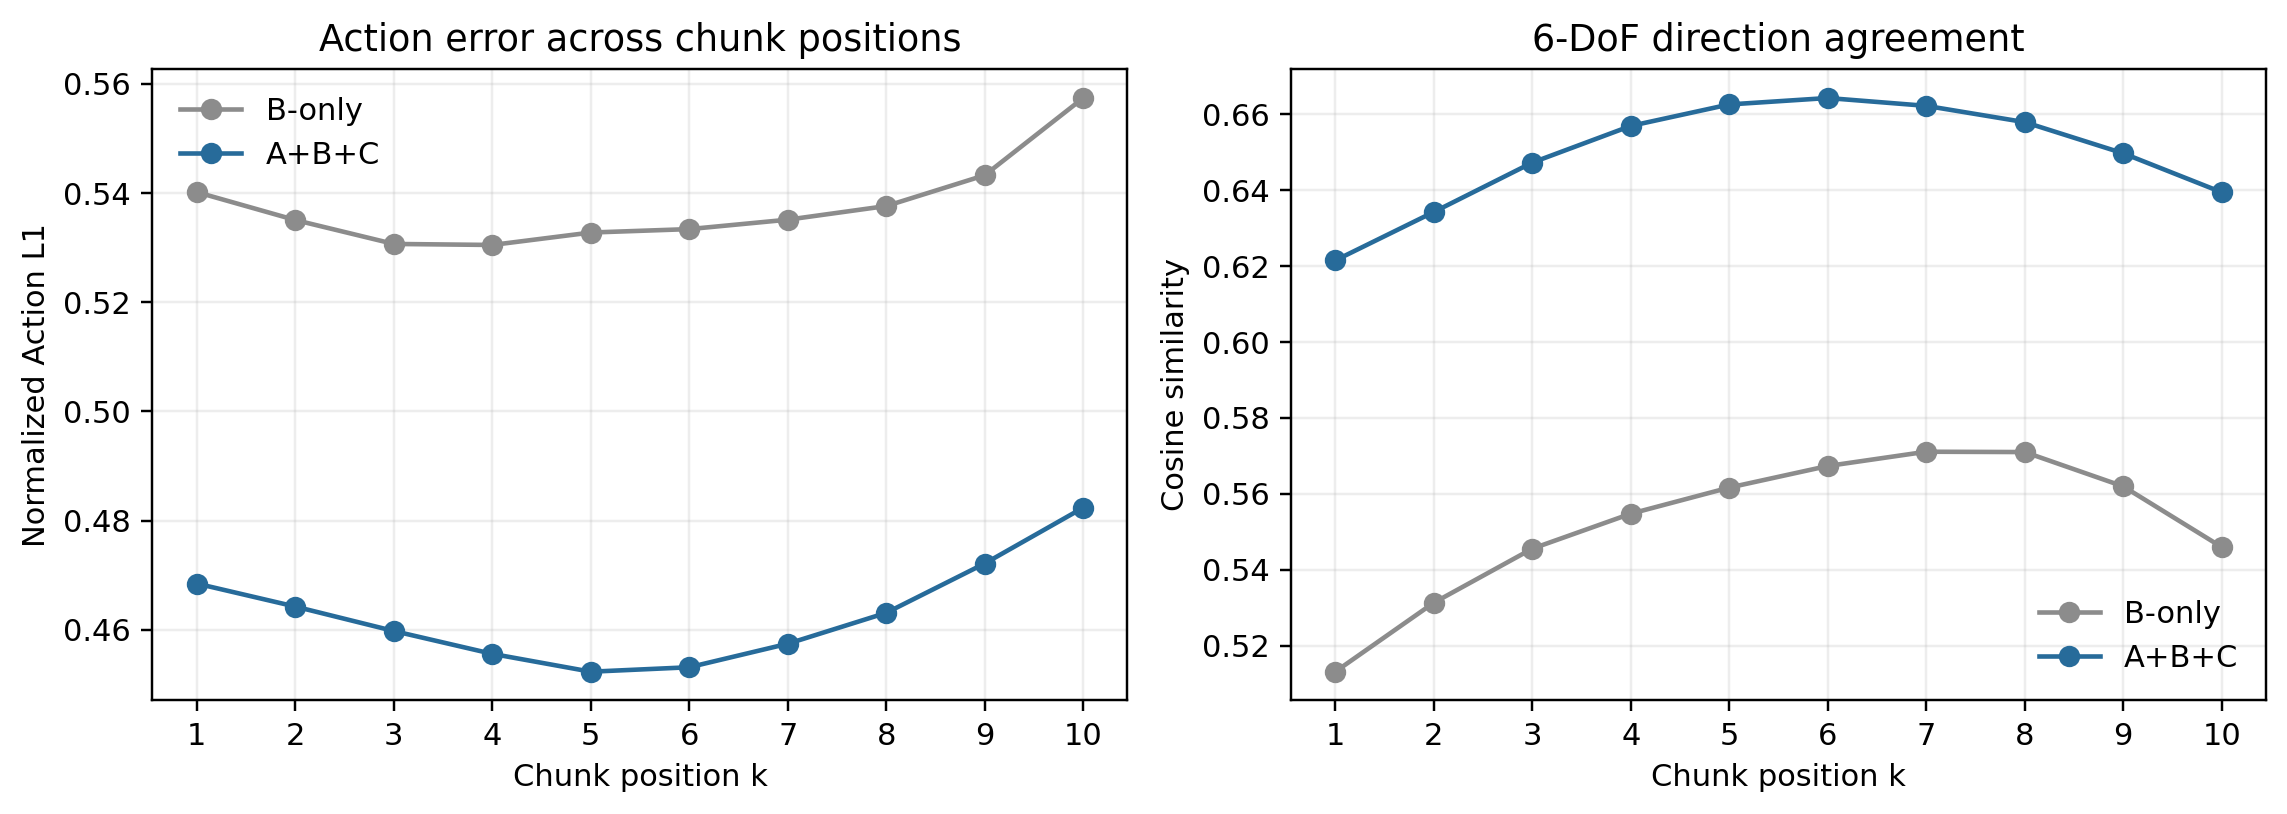
\includegraphics[width=0.96\linewidth]{figures/task2_chunk_horizon.png}
\caption{Clean D 上的 10 步 action chunk 分解。左：每个分块位置的归一化 Action L1；右：机械臂前六维动作方向的余弦相似度。A+B+C 在所有位置都更准确，且方向一致性明显更高。}
\label{fig:chunk}
\end{figure*}

这一结果揭示了固定长度 chunk 的第一层鲁棒性：视觉编码只在 chunk 起点计算一次，十个 query 在同一个视觉上下文下联合产生，因此输出不会像逐步自回归动作预测那样把前一步预测作为下一步网络输入；视觉偏移造成的是整块共同偏差，而不是 chunk 内部的递归数值发散。图~\ref{fig:heatmap} 进一步证明这一点。模糊、噪声、相机平移和遮挡引起的颜色在横向 $k=1\ldots10$ 上大体均匀，误差从第一步开始累积，并没有在第十步突然放大。A+B+C 对相机平移和遮挡的相对退化较大，但同一行内仍然平坦，说明主要问题是视觉表征整体错位，而非动作解码器的远期失衡。

\begin{figure*}[t]
\centering
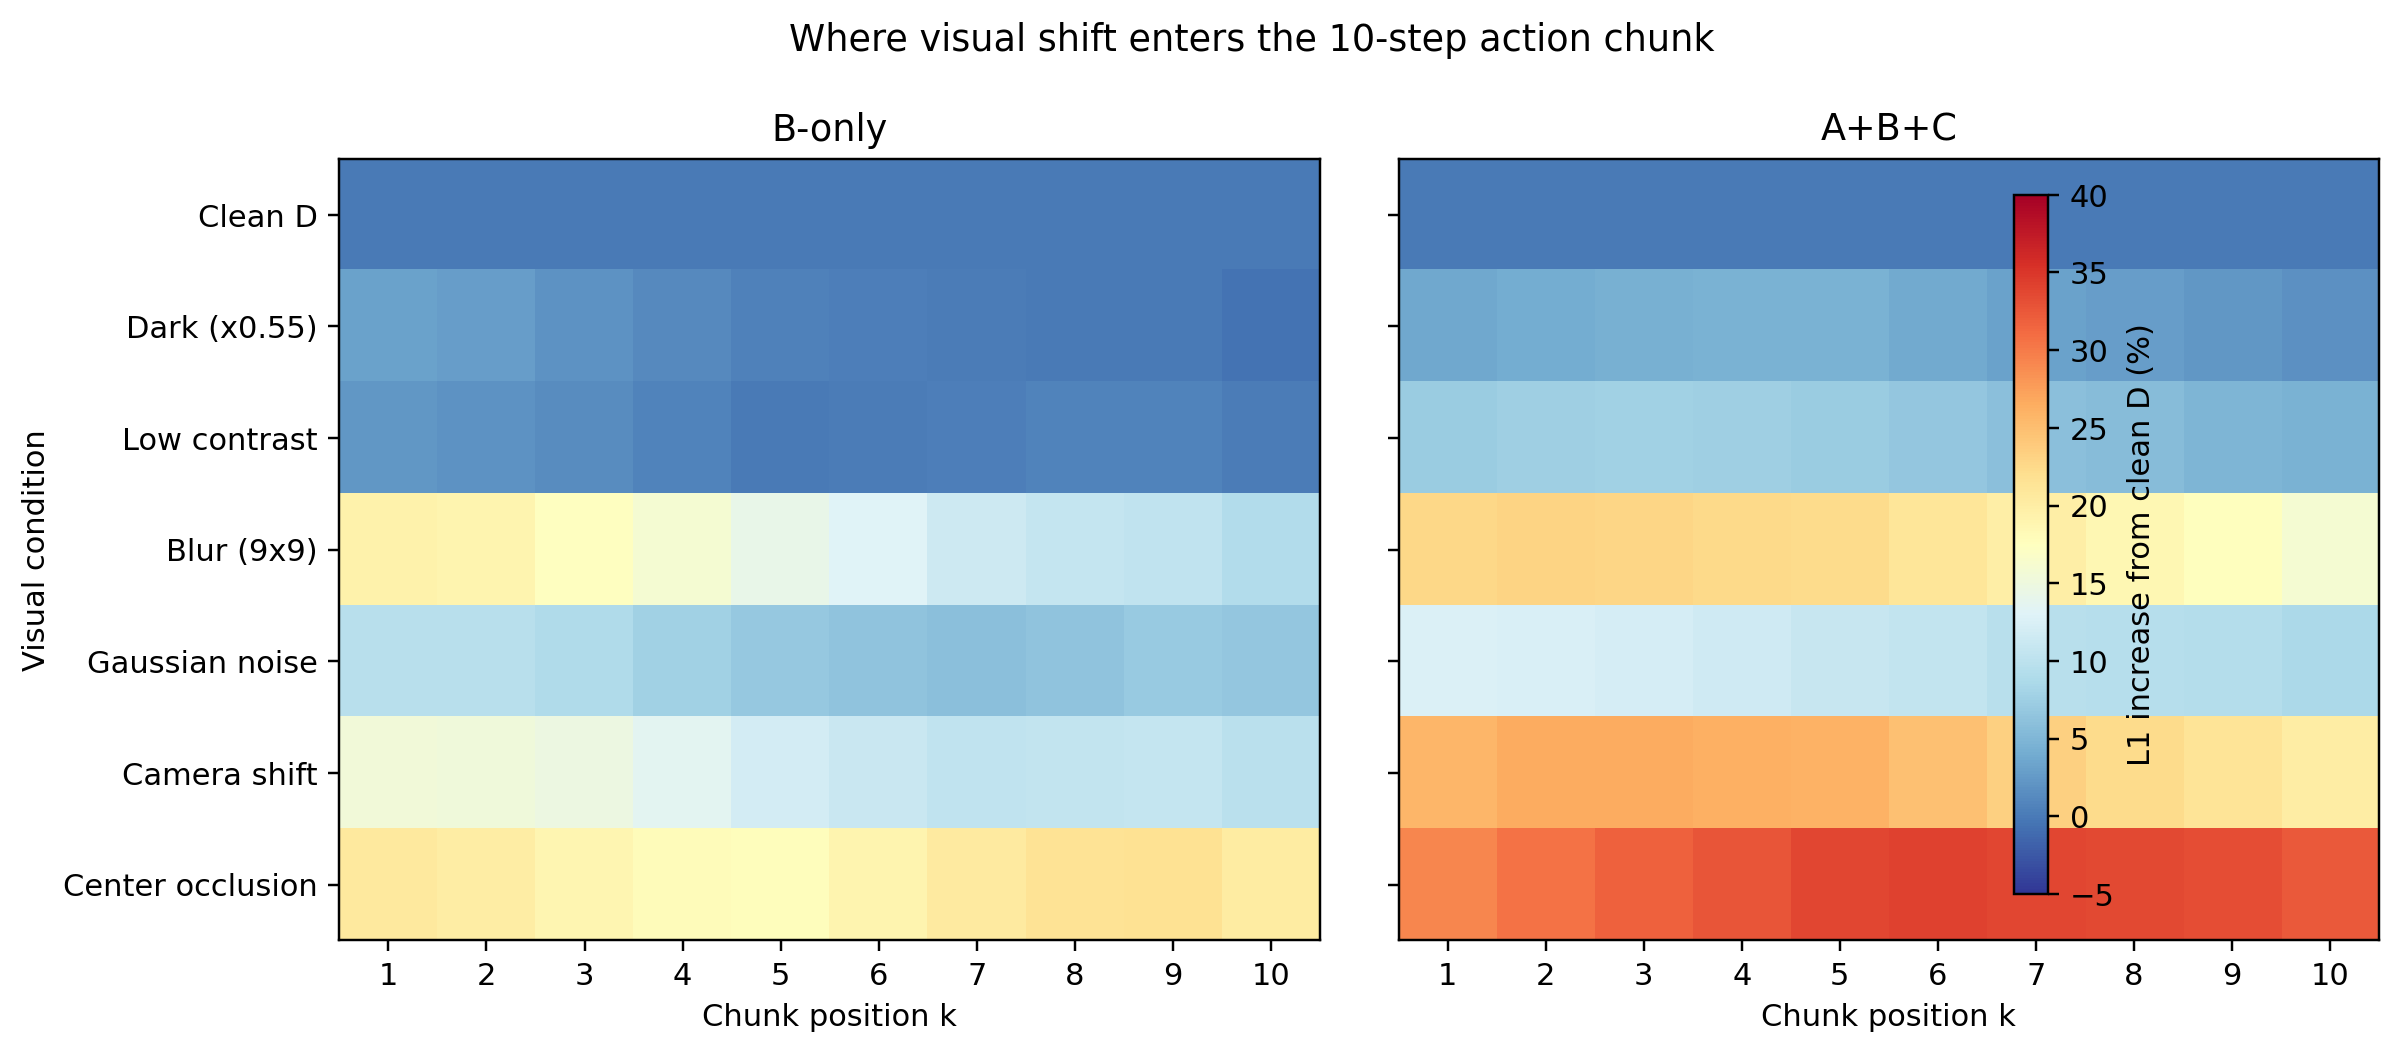
\includegraphics[width=0.96\linewidth]{figures/task2_horizon_shift_heatmap.png}
\caption{视觉扰动在 10 步 chunk 中的位置分布。数值是相对各模型 clean D 的 L1 增幅。大多数扰动从 $k=1$ 起近似均匀影响整块，而不是随分块位置累积。}
\label{fig:heatmap}
\end{figure*}

当前配置会连续执行 10 步且没有 temporal ensemble；如果第一帧视觉判断错误，同一偏差会持续覆盖整个控制块，期间无法利用新观测纠正。固定分块能够提高短时动作一致性并把递归预测误差限制在块边界，但以降低 10 步内反应频率为代价。

\subsection{方向一致性、动态幅度与动作维度}

仅看平均 L1 会混合方向错误、幅度错误和过度平滑。图~\ref{fig:chunk} 右侧显示，A+B+C 的六维机械臂方向余弦相似度均值为 0.650，B-only 为 0.552，绝对提升 0.097，说明联合训练不仅缩小了动作数值，还更可靠地预测了运动方向。夹爪开闭符号准确率由 90.73\% 提高到 92.85\%。

相邻动作差分 L1 由 0.2374 降至 0.2257，但预测/真实时序变化比由 B-only 的 0.507 降至 A+B+C 的 0.406。两者都存在过平滑，A+B+C 的数值更准确、方向更一致，但动态幅度被抑制得更强。这说明多环境训练降低了“连续但错误”的风险，同时也可能通过更保守的动作幅度换取泛化。

\begin{table}[t]
\centering
\caption{Clean D 的动作维度 L1 与 A+B+C 相对改进。}
\label{tab:dims}
\small
\begin{tabular}{lrrr}
\toprule
维度 & B-only & A+B+C & 改进 \\
\midrule
$\Delta x$ & 0.5896 & 0.4559 & 22.68\% \\
$\Delta y$ & 0.5450 & 0.4654 & 14.60\% \\
$\Delta z$ & 0.5264 & 0.4648 & 11.71\% \\
$\Delta roll$ & 0.7448 & 0.6752 & 9.34\% \\
$\Delta pitch$ & 0.6939 & 0.6271 & 9.63\% \\
$\Delta yaw$ & 0.4675 & 0.3999 & 14.47\% \\
gripper & 0.1943 & 0.1504 & 22.61\% \\
\bottomrule
\end{tabular}
\end{table}

表~\ref{tab:dims} 表明 $\Delta x$ 与夹爪改善超过 22\%，其余平移和 yaw 改善约 12--15\%，而 roll/pitch 仍是最难维度，误差最高且收益不足 10\%。视觉分布变化首先破坏物体和末端执行器的空间对应；旋转又比平移更依赖局部接触姿态，因此即使总 L1 改善，精细对准仍是最可能造成实际任务失败的部分。

\subsection{视觉分布偏移的分解}

首先直接比较 B 与 D 的像素统计。静态相机 RGB 直方图 Jensen--Shannon divergence 为 0.00134，均值 RGB 的 L2 距离为 0.01986；腕部相机分别为 0.00334 和 0.04800，约为静态相机的 2.5 倍和 2.4 倍。腕部平均亮度也由 B 的 0.5340 降至 D 的 0.5066。D 与 B 的低层外观差异并不平均分布在两路相机，近场腕部视角承担了更强的 domain shift。

\begin{figure*}[t]
\centering
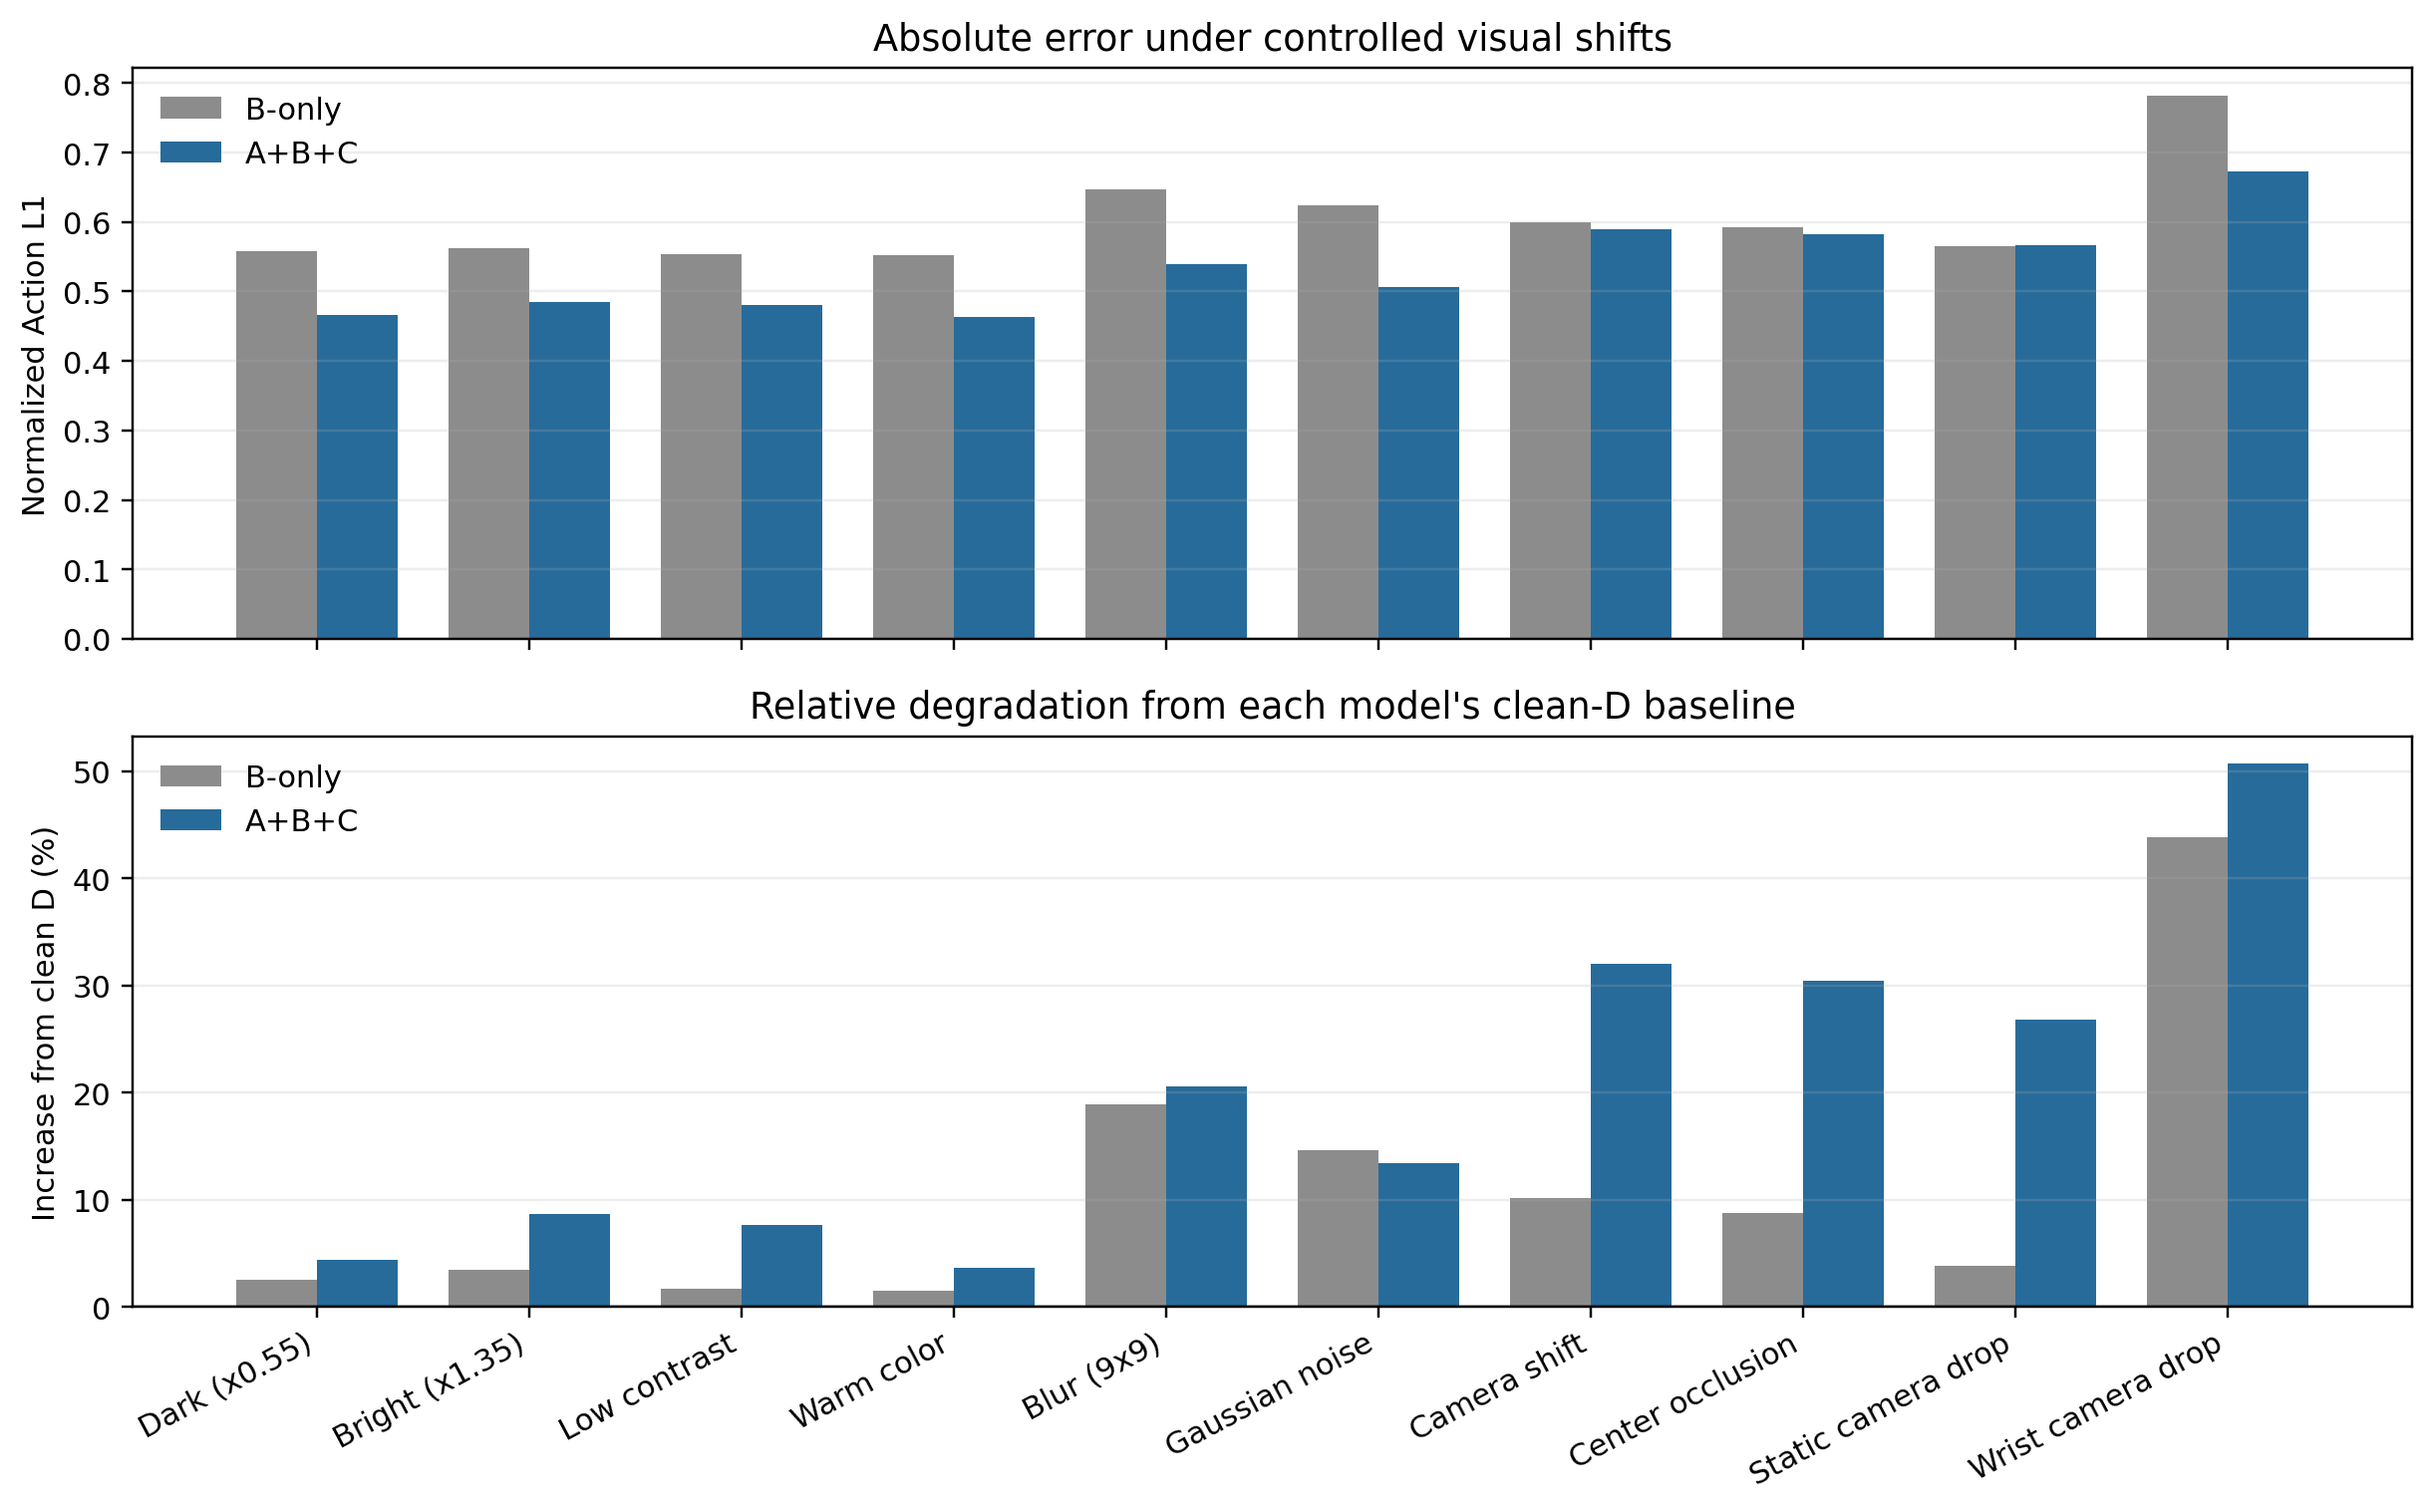
\includegraphics[width=0.96\linewidth]{figures/task2_visual_shifts.png}
\caption{同一批 D 帧上的受控视觉扰动。上：绝对 Action L1，决定哪个模型实际更准确；下：相对各自 clean D 的退化，反映模型对扰动的敏感度。两种视角必须同时使用，避免低基线模型被相对百分比误导。}
\label{fig:shifts}
\end{figure*}

\begin{table}[t]
\centering
\caption{视觉偏移族的平均结果。Adv. 为 A+B+C 相对 B-only 的绝对 L1 优势；Drift 为扰动前后预测变化。}
\label{tab:shiftgroups}
\scriptsize
\setlength{\tabcolsep}{3pt}
\begin{tabular}{lrrrrr}
\toprule
偏移族 & B L1 & ABC L1 & Adv. & B drift & ABC drift \\
\midrule
外观 & 0.5481 & 0.4850 & 11.52\% & 0.1845 & 0.1771 \\
损坏 & 0.5960 & 0.5357 & 10.12\% & 0.3264 & 0.3153 \\
空间 & 0.6240 & 0.5940 & 4.80\% & 0.4380 & 0.4586 \\
相机缺失 & 0.6633 & 0.6312 & 4.85\% & 0.4905 & 0.4849 \\
\bottomrule
\end{tabular}
\end{table}

图~\ref{fig:shifts} 与表~\ref{tab:shiftgroups} 给出三个层次的证据。

\textbf{外观变化。} 暗化、增亮、低对比度和暖色偏移下，A+B+C 平均 L1 为 0.4850，仍比 B-only 的 0.5481 低 11.52\%；其预测漂移也略小。训练环境多样性确实学到了部分光照和颜色不变性。

\textbf{图像损坏。} 模糊和噪声把两模型误差都明显拉高，但 A+B+C 保持 10.12\% 的优势，预测漂移由 0.3264 降至 0.3153。其优势低于 clean D 的 13.90\%，说明多环境训练提高了稳定性，但不能完全抵消局部纹理损坏。

\textbf{空间几何变化。} 相机平移与中心遮挡下，A+B+C 的绝对优势缩小到 4.80\%，预测漂移反而略高于 B-only。具体而言，相机平移与中心遮挡使 A+B+C 相对自身 clean D 分别退化 24.37\% 和 32.43\%。这不是 A+B+C 的绝对误差更差，而是它对固定双相机几何的利用更强，一旦像素位置与训练几何不一致，clean 条件下的优势明显收窄。近期关于相机条件化策略的研究也发现，未显式输入相机外参的 ACT 等 RGB 策略会从静态背景推断视角，换视角后这种捷径会失效~\cite{jiang2025camera}；本实验的空间扰动结果与该机制一致。

\begin{figure*}[t]
\centering
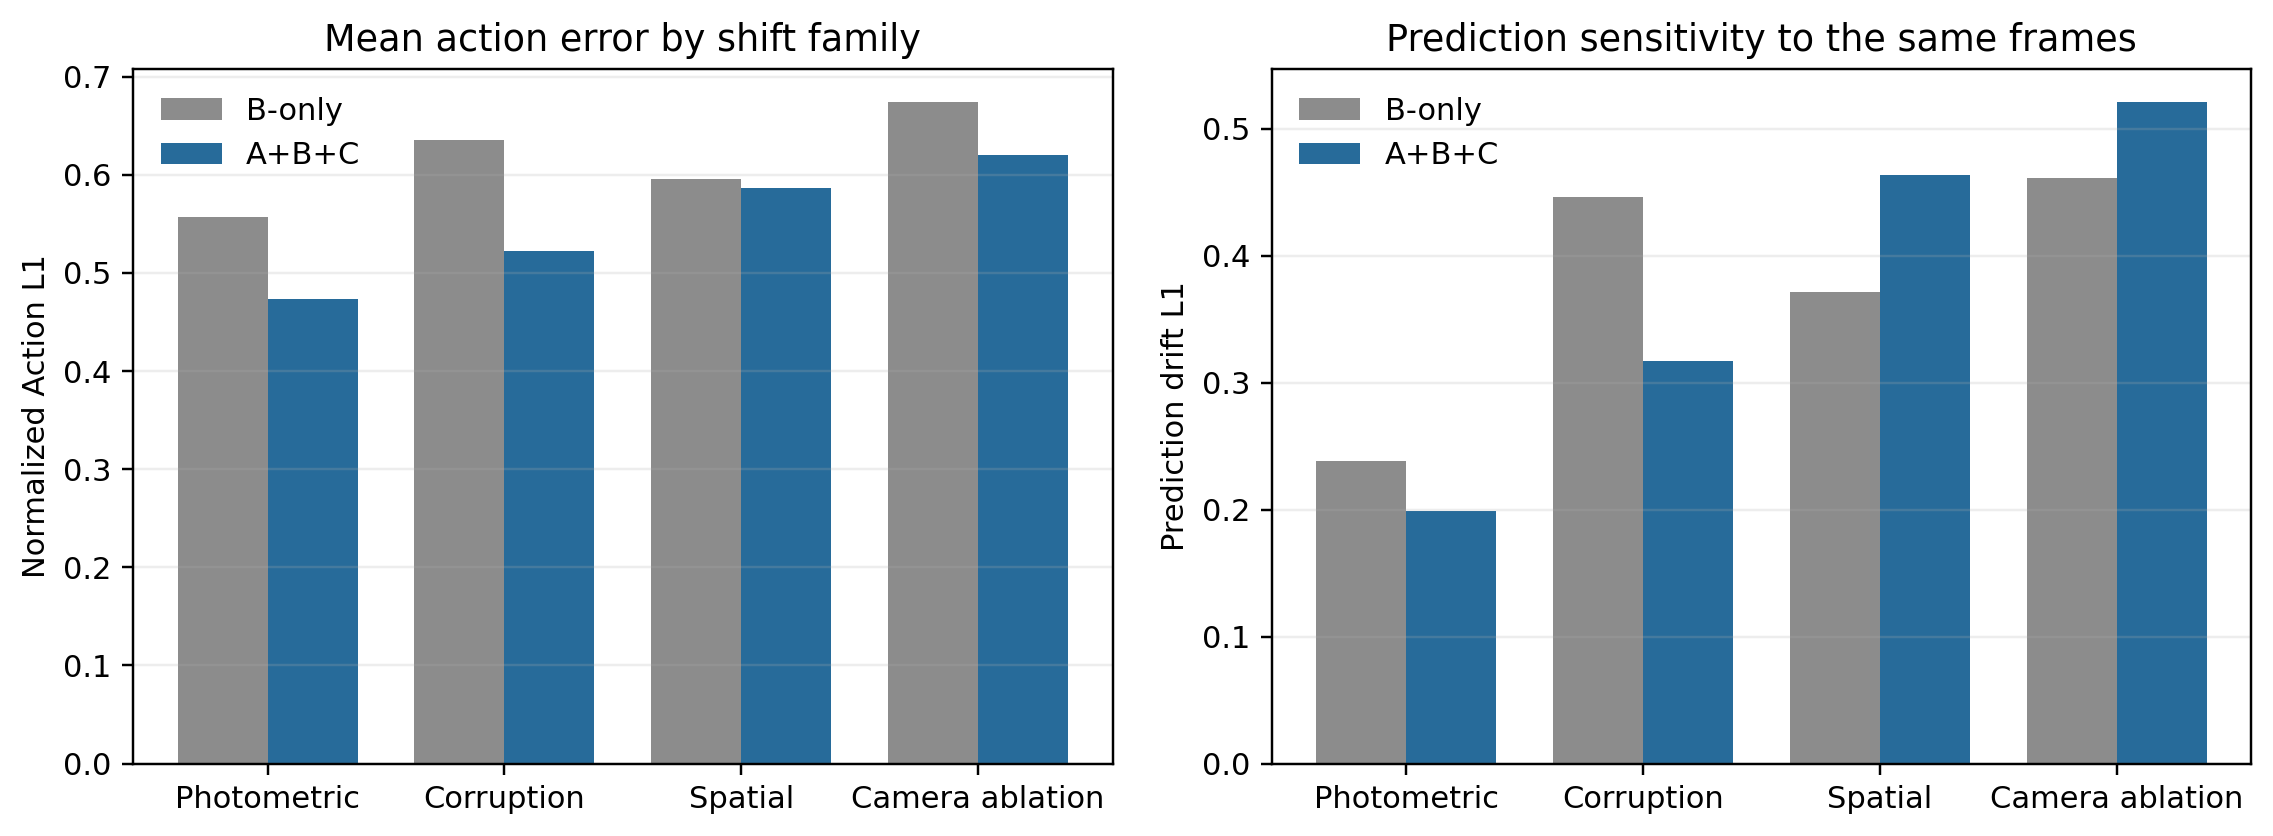
\includegraphics[width=0.92\linewidth]{figures/task2_robustness_summary.png}
\caption{按视觉偏移机制分组的结果。左：绝对动作误差；右：同一帧受扰动前后的预测漂移。A+B+C 在外观和图像损坏上更稳定，但在空间变化和相机缺失上更敏感。}
\label{fig:summary}
\end{figure*}

\subsection{双相机消融与机制解释}

移除静态相机时，B-only 从 0.5374 增至 0.5500，仅退化 2.35\%；A+B+C 从 0.4627 增至 0.5047，退化 9.08\%，但仍保留较低绝对误差。移除腕部相机的影响更严重：B-only 达到 0.7767（$+44.54\%$），A+B+C 达到 0.7576（$+63.75\%$）。结合腕部 B$\rightarrow$D 像素分布差异约为静态视角 2.5 倍，可以判断腕部相机同时是最重要的近场控制来源和最强的 domain-shift 通道。相机缺失时两模型差距显著缩小，说明多环境训练无法替代关键视角本身。

这些结果也解释了 Action Chunking 在视觉偏移下何时有效。对于亮度、颜色、模糊和噪声，只要视觉编码仍能定位目标与末端执行器，联合生成 10 步动作可以保持方向和短时连续性；A+B+C 在每个 $k$ 上都更准确，且误差不随 chunk 尾部放大。对于相机平移、遮挡或相机缺失，问题发生在 chunk 生成之前：视觉 token 已经对应错误位置或缺少关键近场信息，Transformer 会把这个错误条件一致地传播到整个 10 步序列。Action Chunking 能抑制时间上的抖动，却不能自行获得视角不变性。

当前 10 步 ACT 对外观与局部图像损坏具有可量化的短时鲁棒性，但对相机几何偏移没有同等鲁棒性；多环境训练改善了动作表示，却强化了对固定双相机布局的依赖。若继续提升，应优先加入相机位姿随机化或显式外参编码，并把执行长度与预测长度解耦，例如保留 10 步预测但每 1--2 步重新查询，再用 temporal ensemble 融合重叠 chunk。这样才能在维持平滑性的同时恢复对新观测的反应能力。

\section{结论}

任务一的三个正式资产分别遵循题目指定路线。A 的 469 视角白背景 30k 2DGS 测试 PSNR 为 30.40 dB，但可靠方位只有 281.6°；前景支持与异常 footprint 过滤消除了白射线，保真相似变换避免了统一圆盘补丁造成的材质和几何损失，剩余破损可追溯到 78.4° 相机覆盖缺口。B 通过单 prompt、threestudio、SD1.5 和纯 SDS 训练 10000 步得到汉堡，整体层次稳定，局部仍有 SDS 毛刺。C 正式采用 Magic123 v5 fine，双头问题解决，背面仍受单图不可见区域限制。B/C 的带纹理 mesh 通过面积采样、面法线旋转和面积相关 footprint 转成 2D Gaussian；A/B/C 直接追加到背景 GaussianModel，并由一次 rasterizer 调用完成统一深度排序。

任务二中，两模型采用严格对齐的 10k/cosine 协议；A+B+C 在完整 D shard 上比 B-only 的 Action L1 低 15.05\%，配对子集差值的 95\% bootstrap CI 不跨 0。10 步分块的尾部/头部误差比由 1.020 变为 1.018，没有出现随 horizon 快速发散；机械臂方向余弦相似度由 0.552 提升到 0.650。外观和图像损坏下保留约 10--12\% 的绝对误差优势，空间偏移和相机缺失下只剩约 5\%，腕部相机缺失是最严重退化。Action Chunking 的主要收益是短时动作一致性，而不是自动获得相机几何不变性；在当前无 temporal ensemble 的 10 步执行设置中，错误视觉条件会一致地影响整个 chunk。

{\small
\begin{thebibliography}{9}

\bibitem{huang20242dgs}
B. Huang, Z. Yu, A. Chen, A. Geiger, and S. Gao.
\newblock 2D Gaussian Splatting for Geometrically Accurate Radiance Fields.
\newblock \emph{ACM Transactions on Graphics}, 2024.

\bibitem{guedon2024sugar}
A. Gu\'edon and V. Lepetit.
\newblock SuGaR: Surface-Aligned Gaussian Splatting for Efficient 3D Mesh Reconstruction and High-Quality Mesh Rendering.
\newblock In \emph{CVPR}, 2024.

\bibitem{qian2023magic123}
G. Qian, J. Mai, A. Hamdi, J. Ren, I. Skorokhodov, P. Wonka, S. Tulyakov, and B. Ghanem.
\newblock Magic123: One Image to High-Quality 3D Object Generation Using Both 2D and 3D Diffusion Priors.
\newblock \emph{arXiv:2306.17843}, 2023.

\bibitem{poole2022dreamfusion}
B. Poole, A. Jain, J. T. Barron, and B. Mildenhall.
\newblock DreamFusion: Text-to-3D using 2D Diffusion.
\newblock In \emph{ICLR}, 2023.

\bibitem{barron2022mipnerf360}
J. T. Barron, B. Mildenhall, D. Verbin, P. P. Srinivasan, and P. Hedman.
\newblock Mip-NeRF 360: Unbounded Anti-Aliased Neural Radiance Fields.
\newblock In \emph{CVPR}, 2022.

\bibitem{zhao2023act}
T. Z. Zhao, V. Kumar, S. Levine, and C. Finn.
\newblock Learning Fine-Grained Bimanual Manipulation with Low-Cost Hardware.
\newblock In \emph{Robotics: Science and Systems}, 2023.

\bibitem{mees2022calvin}
O. Mees, L. Hermann, E. Rosete-Beas, and W. Burgard.
\newblock CALVIN: A Benchmark for Language-Conditioned Policy Learning for Long-Horizon Robot Manipulation Tasks.
\newblock \emph{IEEE Robotics and Automation Letters}, 2022.

\bibitem{xie2023generalization}
A. Xie, L. Lee, T. Xiao, and C. Finn.
\newblock Decomposing the Generalization Gap in Imitation Learning for Visual Robotic Manipulation.
\newblock In \emph{IEEE International Conference on Robotics and Automation}, 2024.

\bibitem{jiang2025camera}
T. Jiang, J. Ji, X. Tan, J. Fang, A. Bhattad, V. Guizilini, and M. R. Walter.
\newblock Do You Know Where Your Camera Is? View-Invariant Policy Learning with Camera Conditioning.
\newblock \emph{arXiv:2510.02268}, 2025.

\end{thebibliography}
}

\end{document}
